%%% Local Variables:
%%% mode: latex
%%% TeX-master: t
%%% End:
\chapter{基于模式解耦的弹性波最小平方逆时偏移}
\label{cha:MD-ELSRTM}
\section{引言}
前一章内容中我们将模型分解为高波数与低波数成分,并通过弹性波WERTI方式来恢复模型的低波数成分。常规的FWI算法可以恢复模型的高波数成分,但是会受到许多因素干扰,
如cycle-skipping问题,信噪比低,地震子波未知,正演算子不准确等等。除此之外,我们通常也会通过最小平方偏移(LSM)来实现高波数成分的重构。
早在1993年,Schuster(1993)\cite{Schuster1993}提出了针对井间数据的LSM算法,而Nemeth et al.\cite{Nemeth1999}将该方法应用到了地面数据中。
以波动方程为引擎的最小平方逆时偏移(LSRTM)近年来一直是研究的热点,例如Dai and
Schuster(2013)\cite{Dai2013},Dong et al.(2012)\cite{Dong2012}, Luo and
Hale(2014)\cite{Luo2014}。尽管其计算代价昂贵,但是LSRTM可以回避模型速度复杂时所产生的多路径问题。
LSRTM的过程通常被认为是线性的全波形反演,其假设在已经获得足够好的低波数模型成分之后恢复模型的高频扰动,也即获得“像”,使得在最小平方意义下,
用该“像”所预测的反射数据能与观测数据达到最佳匹配。因此,最小平方逆时偏移与全波形反演的理论框架是一致的。

近期,为了更准确地描述波传播过程,同时获得更多的参数
成像,并解决多参数带来的耦合效应,原本基于声波方程的
LSRTM被推广到了变密度声波介质\cite{Yang2017},衰减介质\cite{Dai2015}以及弹性介质中\cite{Duan2016,Feng2016,Xu2016}(ELSRTM)。
相比声波成像,弹性波成像可以提供更多的地下信息,例如裂缝分布以及弹性性质。但是,弹性波偏移中存在的许多问题会很大程度上影响成像质量。因为通常很难将记录中的
波模式完全区分开,因此其中某些波模式的会因速度不对而被错误地成像。这些非物理的模式就会引起假象,也即“cross-talk”。
而通过ELSRTM则可以提高成像的分辨率,并且可以压制由于观测孔径限制,粗网格采样以及数据缺失引起的偏移假象。
弹性波成像需要处理矢量波的问题,也就需要选取合适的成像条件,{\color{red}\cite{Wang2016}提出了无极性反转的矢量成像条件等等。}而从EFWI理论框架出发,许多学者,
如Duan et al.(2016)\cite{Duan2016},Feng et
al.(2016)\cite{Feng2016}等都推导出了与EFWI梯度非常类似的成像条件。该成像条件也可以回避极性反转问题,同时也可以认为是更加接近于高频的参数扰动梯度。而基于
第二章中对EFWI算法的分析,模式解耦带来的优势将同样能在ELSRTM中得以应用,因此我们将在本章中应用波模式解耦来对ELSRTM进行预条件,从而获得更好结果。
\section{矩阵形式弹性波方程}
与第二章中类似,我们将从弹性波方程出发,推导出E-LSRTM的梯度。本章中,为了方便,我们同样将在频率域
利用矩阵形式的弹性波方程来完成推导。方程\ref{eq:WE}可以写作:
\begin{equation}
\mathbf{L}(\lambda,\mu,\rho)\mathbf{U}=\mathbf{f},
    \label{eq:WE_Matrix} 
\end{equation}
其中,位移场与应力场构成波场矢量满足$\mathbf{U}=[u_x,u_z,\tau_{xx},\tau_{zz},\tau_{xz}]^T$,$\mathbf{f}$为震源,并且
\begin{equation}
        \mathbf{L}=
        =
        \begin{bmatrix}
%			&\rho\partial^2_{tt} &0 &-\partial_x & 0 &-\partial_z\\
			&-\rho\omega^2 &0 &-\partial_x & 0 &-\partial_z\\
			& 0  &-\rho\omega^2 &0 &-\partial_z &-\partial_x\\
%			& 0  &\rho\partial^2_{tt} &0 &-\partial_z &-\partial_x\\
			&-(\lambda+2\mu)\partial_x &-\lambda\partial_z &1 &0&0\\
			& -\lambda\partial_x  &-(\lambda+2\mu)\partial_z &0 &1&0\\
			& -\mu\partial_z  &-\mu\partial_x &0 &0&1\\
        \end{bmatrix},
        \label{eq:L}
\end{equation}
上式中$\omega$为角频率,$\partial_x$和$\partial_z$分别为空间x和z方向一阶导数,$\rho,\lambda,\mu$为弹性介质背景参数。在有模型扰动
$\delta\lambda,\delta\mu,\delta\rho$时,介质中总波场和扰动场满足:
\begin{equation}
\mathbf{L}(\lambda+\delta\lambda,\mu+\delta\mu,\rho+\delta\rho)(\mathbf{U+\delta U})=\mathbf{f},
    \label{eq:WE_Matrix_all} 
\end{equation}
将式\ref{eq:WE_Matrix_all}减去式\ref{eq:WE_Matrix}则可得扰动波场与背景波场之间的关系:
\begin{equation}
\mathbf{L}(\lambda,\mu,\rho)\mathbf{\delta U}=-\mathbf{L}^{'}\mathbf{U},
    \label{eq:WE_Matrix_delta} 
\end{equation}
其中$\mathbf{L}^{'}=(\delta\lambda\mathbf{L}^{'}_{\lambda}+\delta\mu\mathbf{L}^{'}_{\mu}+\delta\rho\mathbf{L}^{'}_{\rho})$,且
\begin{equation}
        \mathbf{L}^{'}_{\lambda}=
        \begin{bmatrix}
			&0 &0 &0 & 0 &0\\
			& 0  &0 &0 &0 &0\\
			&-\partial_x &-\partial_z &0 &0&0\\
			& -\partial_x  &-\partial_z &0 &0&0\\
			& 0  &-0&0 &0&0\\
        \end{bmatrix},
%        \label{eq:L_lambda}
        \mathbf{L}^{'}_{\mu}=
        \begin{bmatrix}
            &0 &0 &0 & 0 &0\\
            & 0  &0 &0 &0 &0\\
            &-2\partial_x &0 &0 &0&0\\
            & 0  &-2\partial_z &0 &0&0\\
            & -\partial_z  &-\partial_x&0 &0&0\\
        \end{bmatrix},
        \label{eq:L_lambdamu}
\end{equation}
\begin{equation}
        \mathbf{L}^{'}_{\rho}=
        \begin{bmatrix}
		&-\omega^2 &0 &0 & 0 &0\\
            & 0  &-\omega^2 &0 &0 &0\\
            &0&0 &0 &0&0\\
            &0  &0 &0 &0&0\\
            & 0  &-0&0 &0&0\\
        \end{bmatrix}.
        \label{eq:L_rho}
\end{equation}
由于在E-LSRTM中假设背景场及背景模型不发生变化,则可将方程\ref{eq:WE_Matrix_delta}看作为新的状态方程,
方程右端项为背景波场与参数扰动之间通过辐射模式作用形成新的震源。
上述问题通常假定在背景模型足够好的时候来恢复扰动,因此方程也只描述一次散射。
与EFWI中所描述的正问题不同的是,该正问题只考虑反射(散射)波的扰动而不包含透射波(直达波)。
然而实际地下介质中,模型复杂时多次散射效应会对成像带来很大影响。近期,也有学者考虑在该过程中将扰动量同时加入背景场,
例如Guo and
Alkhalifah(2016)\cite{Guo2016}所展示的RWI过程中,他们将界面扰动同时加入到背景场中来包括多次散射效应的影响。
\section{E-LSRTM梯度}
E-LSRTM中我们同样利用$L_2$范数来定义目标函数:
\begin{equation}
    E=\frac{1}{2}\sum_{\omega}\sum_{s,r}\left\lVert \mathfrak{F}\delta \mathbf{U}-\mathbf{d}^{obs} \right \rVert^2,
    \label{eq:misfit_LSRTM}
\end{equation}
其中,$\mathfrak{F}$为重采样函数,$\delta\mathbf{U}$为模拟的反射波数据,$s,r$代表在炮点$s$出发到达接收点$r$的炮检关系
,该目标函数要对所有频率所有炮检对的反射数据残差求和。利用lagrangian乘子法,建立增广函数:
\begin{equation}
\begin{split}
    \mathcal{L}(\delta\mathbf{U},\bm\Psi,\delta\lambda,\delta\mu,\delta\rho)=&Re\left[
	\frac{1}{2}\sum_{\omega}\sum_{s,r}\left\lVert \mathfrak{F}\delta \mathbf{U}-\mathbf{d}^{obs} \right \rVert^2 \right. \\
	&\left.-\sum_{\omega}\sum_{s}\langle\bm\Psi,\mathbf{L}\delta\mathbf{U}-\mathbf{L}^{'}\mathbf{U}\rangle_{\mathbf{x}}\right],
    \label{eq:Lagrangian_LSRTM}
\end{split}
\end{equation}
这里,$\bm\Psi=(\psi_x,\psi_z,\psi_{xx},\psi_{zz},\psi_{xz})^T$为伴随波场,$\langle\rangle_\mathbf{x}$
代表空间域的内积运算,根据Plessix(2006)\cite{plessix2006},该优化问题的极值点需要满足
$\frac{\partial\mathcal{L}}{\partial(\delta\mathbf{U}_s)}=0$,也即对应于共轭状态方程:
\begin{equation}
	\mathbf{L}^*(\lambda,\mu,\rho)\bm\Psi_s=\sum_{r}(\delta\mathbf{U}-\mathbf{d}^{obs}),
    \label{eq:Adjoint_LSRTM} 
\end{equation}
由于每一炮每一个频率的数据都对应一个共轭方程,因此上式中未出现对频率及炮点的求和。为了简单,我们隐去了上式中的重采样函数。上式左端项中
$\mathbf{L}^*$,该共轭转置代表了传播算子的逆时反传,而右端项则代表了每炮数据检波点处的残差波场,因此伴随波场$\bm\Psi$是以数据残差为震源的逆时
传播波场。
则式\ref{eq:Lagrangian_LSRTM}对应的梯度应为:
\begin{equation}
    \frac{\partial\mathcal{L}}{\partial \delta\mathbf{m}}=Re\left(\sum_{\omega}\sum_{s,r}
	\langle\bm\Psi,\frac{\partial \mathbf{L}^{'}}{\partial\delta\mathbf{m}}\mathbf{U}\rangle\right),
    \label{eq:Gradient_LSRTM}
\end{equation}
其中$\delta\mathbf{m}=(\delta\lambda, \delta\mu,\delta\rho)$,
注意到$\frac{\partial\mathcal{L}}{\partial \delta\mathbf{m}}$的相关导数正好对应于,$\frac{\partial\mathcal{L}}{\partial 
\delta\lambda}=\mathcal{L}^{'}_{\lambda}$,$\frac{\partial\mathcal{L}}{\partial\delta\mu}=\mathcal{L}^{'}_{\mu}$以及
$\frac{\partial\mathcal{L}}{\partial\delta\rho}=\mathcal{L}^{'}_{\rho}$。
利用式\ref{eq:L_lambdamu}-\ref{eq:L_rho}对$\delta\mathbf{m}$求导并将其转换到时间域
可得:
\begin{equation}
\begin{split}
   & \frac{\partial\mathcal{L}}{\partial \delta\lambda}=\sum_{s,r}\int^T_{0}
	(\frac{\partial u_x}{\partial x}+\frac{\partial u_z}{\partial z})(\psi_{xx}+\psi_{zz}),\\
   & \frac{\partial\mathcal{L}}{\partial \delta\mu}=\sum_{s,r}\int^T_{0}
	2(\frac{\partial u_x}{\partial x}\psi_{xx}+\frac{\partial u_z}{\partial z}\psi_{zz})+
	(\frac{\partial u_x}{\partial z}+\frac{\partial u_x}{\partial z})\psi_{xz},\\
   & \frac{\partial\mathcal{L}}{\partial \delta\rho}=\sum_{s,r}\int^T_{0}
	\frac{\partial^2 u_x}{\partial t^2}\psi_x+\frac{\partial^2 u_z}{\partial t^2}\psi_{z}.
    \label{eq:Gradient_lambdamurho_LSRTM}
\end{split}
\end{equation}
另外需要注意到的是,将式\ref{eq:Adjoint_LSRTM}变换到时空域并展开:
\begin{equation}
\begin{split}
   & \rho\frac{\partial^2 \psi_{x}}{\partial t^2}=	(\lambda+2\mu)\frac{\partial \psi_{xx}}{\partial x}+
		\lambda\frac{\partial \psi_{zz}}{\partial x}+\mu\frac{\partial \psi_{xz}}{\partial z},\\
   & \rho\frac{\partial^2 \psi_{z}}{\partial t^2}=	\lambda\frac{\partial \psi_{xx}}{\partial z}+
		(\lambda+2\mu)\frac{\partial \psi_{zz}}{\partial z}+\mu\frac{\partial \psi_{xz}}{\partial x},\\
   & \psi_{xx}=\frac{\partial \psi_x}{\partial x}, \psi_{zz}=\frac{\partial \psi_z}{\partial z},\\
   & \psi_{xz}=\frac{\partial \psi_x}{\partial z} + \frac{\partial \psi_z}{\partial x},
    \label{eq:Time_Adjoint_WE_LSRTM}
\end{split}
\end{equation}
可以看到在反传波场的求取过程中,由于转置算子的作用导致伴随状态方程发生了改变不再是原本的弹性波方程,新的方程中多出了两项应力导数项,同时应力
应变也不再是原本的关系,这是求解中需要注意的。但是我们也通过实验发现,采用新的方程也并未带来非常大的不同,可以说新方程在数学导出上不一样,但是
不影响物理过程。
\section{模式解耦对E-LSRTM进行预条件}
可以看到以上梯度表达式与EFWI中的梯度(式\ref{eq:DeGradient_vpvsrho})非常类似,只是EFWI中$\lambda$和$\mu$的梯度互相关波场都为位移的空间导数,而
此处则为位移场空间导数与应力场的互相关,密度的梯度表达式则完全一致。
采用速度-密度的参数化方式,我们可以导出$V_p$与$V_s$的E-LSRTM梯度:
\begin{equation}
\begin{split}
   & \frac{\partial\mathcal{L}}{\partial \delta V_p}=2\rho V_p\frac{\partial\mathcal{L}}{\partial \delta \lambda}\\
   & \frac{\partial\mathcal{L}}{\partial \delta V_s}=2\rho V_s(-2\frac{\partial\mathcal{L}}{\partial \delta \lambda}
	+\frac{\partial\mathcal{L}}{\partial \delta \mu})\\
   & \frac{\partial\mathcal{L}}{\partial \delta\rho_{vel}}=(V^2_p-2V^2_s)\frac{\partial\mathcal{L}}{\partial \delta \lambda}+V^2_s\frac{\partial\mathcal{L}}{\partial \delta \lambda}+\frac{\partial\mathcal{L}}{\partial \delta\rho}.
    \label{eq:Gradient_VpVsrho_LSRTM}
\end{split}
\end{equation}

为了利用解耦来降低$V_p$和$V_s$之间的耦合性,我们同样在E-LSRTM中暂不考虑密度扰动。
则考虑模式解耦的E-LSRTM梯度为:
\begin{equation}
\begin{split}
   & \frac{\partial\mathcal{L}}{\partial \delta V_p}=2\rho V_p\sum_{s,r}\int^T_{0}
	(\frac{\partial u_x}{\partial x}+\frac{\partial u_z}{\partial
	z})(\psi_{xx}+\psi_{zz})dt,\\
   & \frac{\partial\mathcal{L}}{\partial \delta V_s}=2\rho V_s\sum_{s,r}\int^T_{0}
	2(\frac{\partial u^M_x}{\partial x}\psi^S_{xx}+\frac{\partial u^M_z}{\partial z}\psi^S_{zz})+
	(\frac{\partial u^M_x}{\partial z}+\frac{\partial u^M_x}{\partial
	z})\psi^S_{xz}dt,
    \label{eq:Gradient_lambdamurho_LSRTM}
\end{split}
\end{equation}
其中$M\in{P,S}$。需要注意到,与EFWI所不同的是LSRTM中我们希望获得高分辨率的高波数分量,因此所处理的数据频率通常较高。但是
在高频数据中,在模型复杂区域,层间多次波或者多次散射经常也会比较严重。尤其是在利用S波波场进行LSRTM的情况下,本身S波波场能量较弱,
对于S波散射或者多次转换严重的区域会对解耦之后的梯度产生很不利的干扰。因此对正传波场的解耦
也会有助于减少假象与干扰。所以这里我们不再约束只对反传播场进行解耦而是否解耦正传波场需要视情况而定。如果多次散射较弱,那么不用解耦正传波场,
如果多次散射严重,就解耦正传波场用更多计算量来压制假象。

此外,前文中也提到需要对梯度进行其他预条件才能更好的加速收敛,这里我们采用震源波场的照明能量来进行补偿:
\begin{equation}
	\mathbf{Q} =\left[\int^T_0(u^2_x+u^2_z)dt\right]^{-1},
    \label{eq:Gradient_Illumination_LSRTM}
\end{equation}
该能量补偿相当于对角Hessian的作用,因此最终采用模式解耦作为预条件的E-LSRTM更新方式如下:
\begin{equation}
        \delta\mathbf{m}_{k+1}=\delta\mathbf{m}_{k}-\alpha_k
        \begin{bmatrix}\mathbf{Q}{\frac{\partial\mathcal{L}}{\partial \delta V_p}}\\
		\mathbf{Q}{\frac{\partial\mathcal{L}}{\partial \delta V_s}}\end{bmatrix}_{k},
        \label{eq:Gradientmethod}
\end{equation}
其中$\delta\mathbf{m}_{k}$为$k$次迭代的模型扰动,$\alpha$为k+1次迭代的步长。
步长搜索我们同样采用抛物线拟合的方式来求取。
\section{数值实验}
\subsection{反射数据与Born数据的差异}
\begin{figure}
   \centering
   \subfloat[]{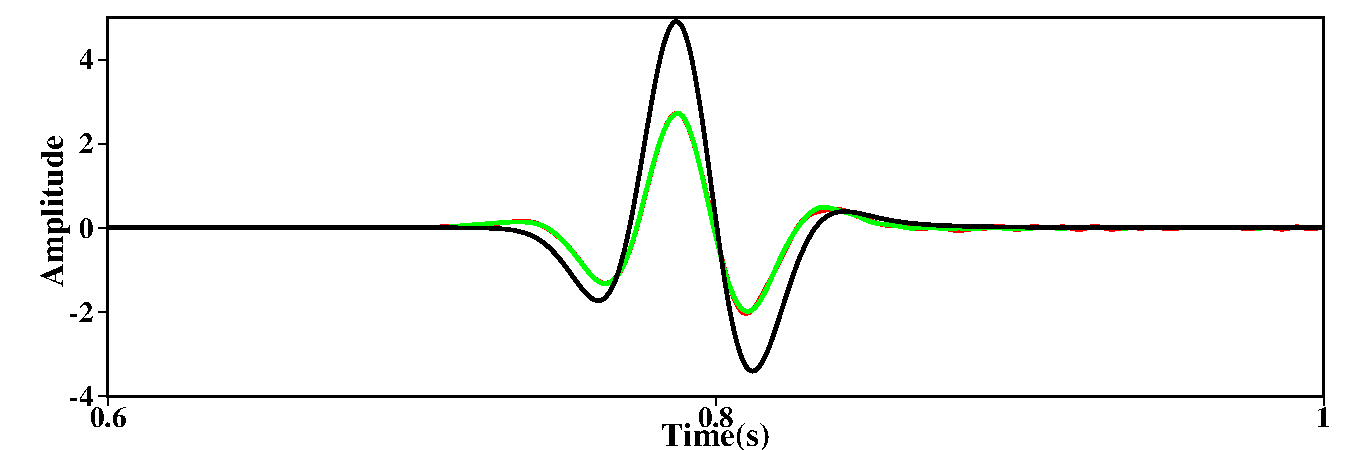
\includegraphics[width=0.58\textwidth]{Figure/chapter04/singlelayer/smooth3.pdf}}\\
   \subfloat[]{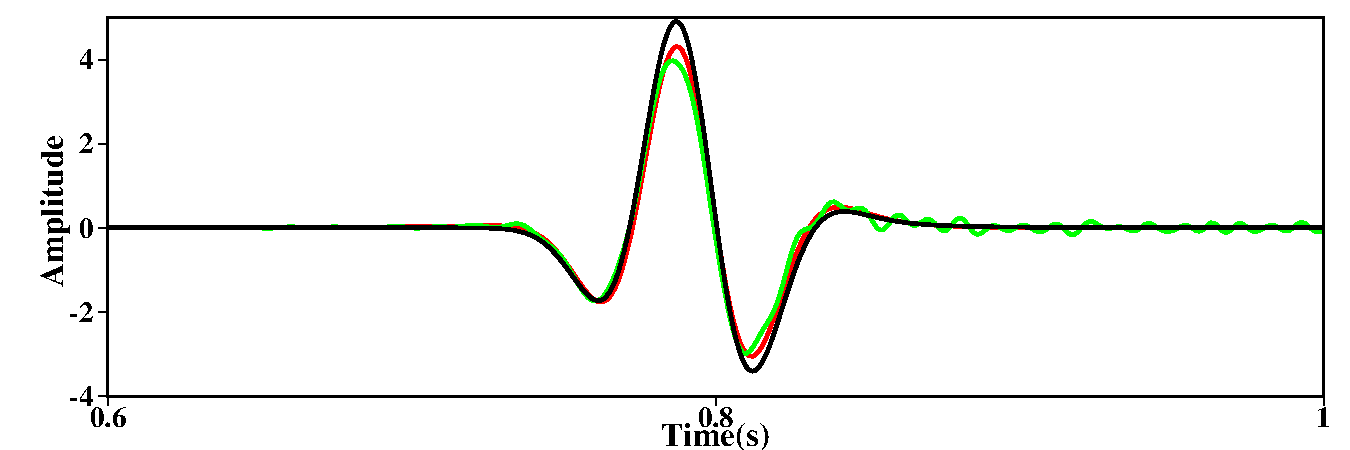
\includegraphics[width=0.58\textwidth]{Figure/chapter04/singlelayer/smooth8.pdf}}
   \caption{Sigbee2A model example. On the top are true models of 
   $V_p$ (a) and $V_s$ (b). On the bottom are initial models of $V_p$ (c) and $V_s$
   (d) linearly increasing with depth. }
   \label{fig:refl_born_comparison}
\end{figure}
\begin{figure}
   \centering
%   \subfloat[]{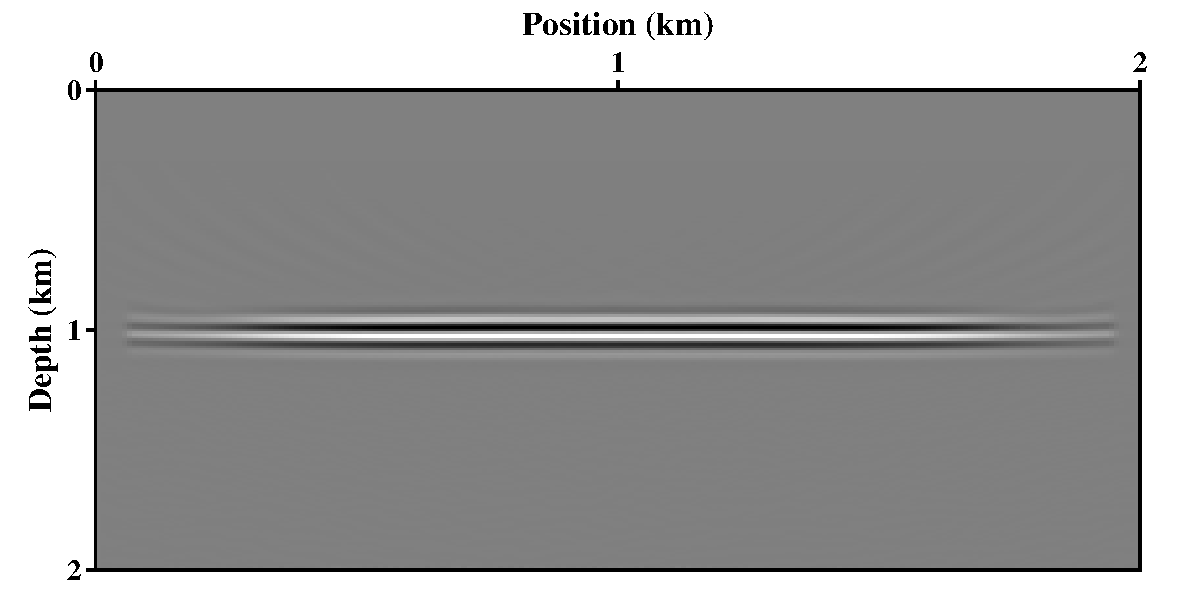
\includegraphics[width=0.48\textwidth]{Figure/chapter04/singlelayer/RTMborn.pdf}}
%   \subfloat[]{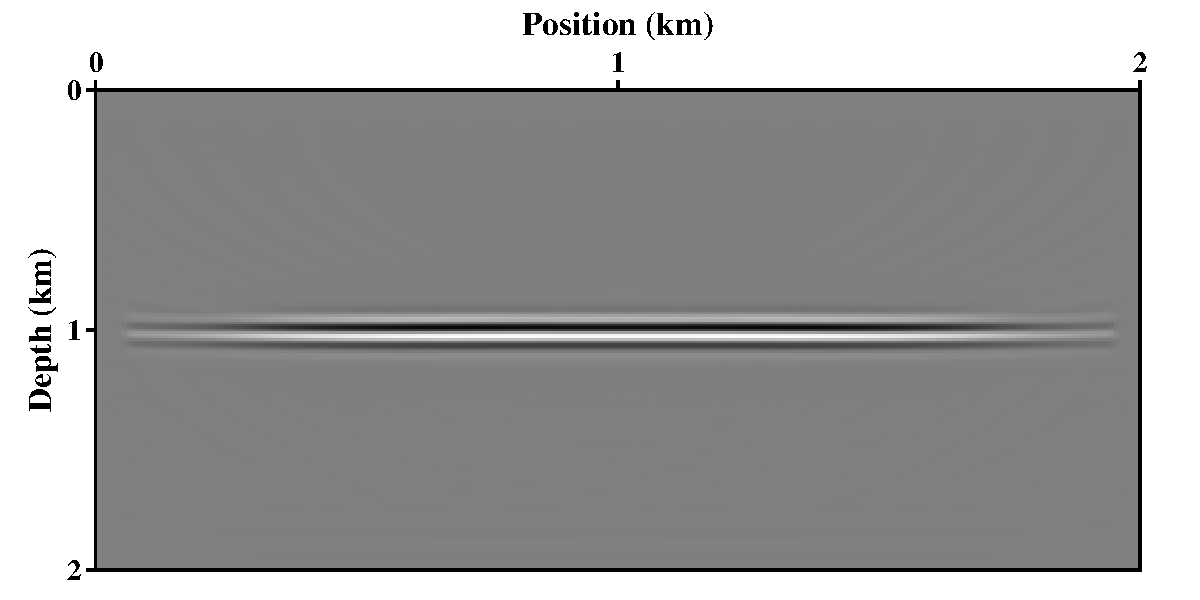
\includegraphics[width=0.48\textwidth]{Figure/chapter04/singlelayer/RTMref.pdf}}\\
   \subfloat[]{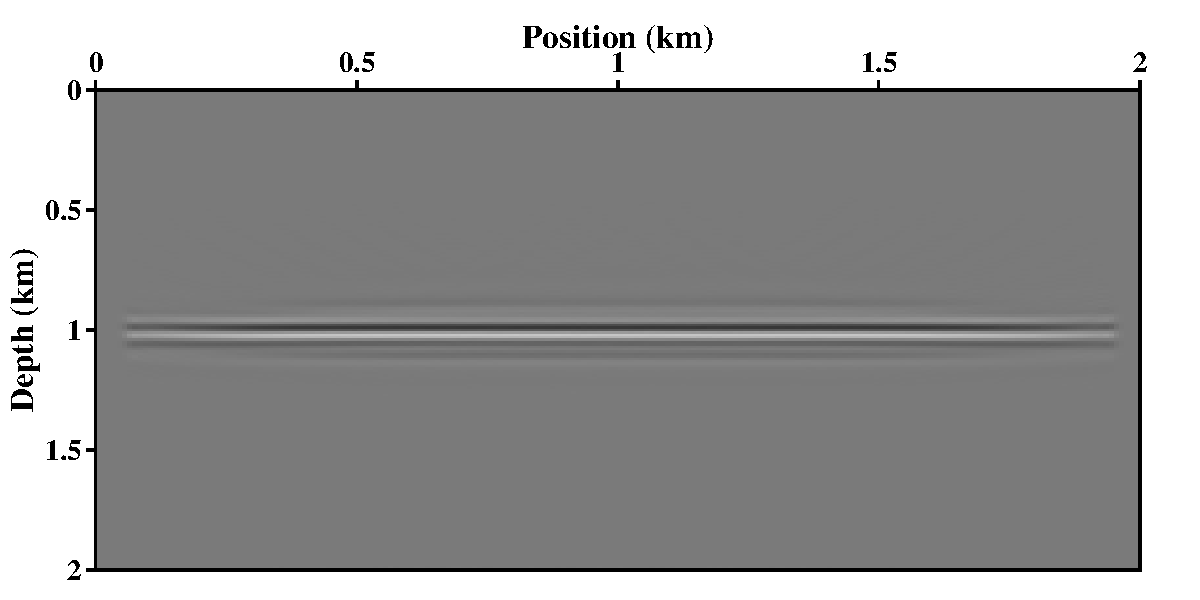
\includegraphics[width=0.48\textwidth]{Figure/chapter04/singlelayer/born.pdf}}
   \subfloat[]{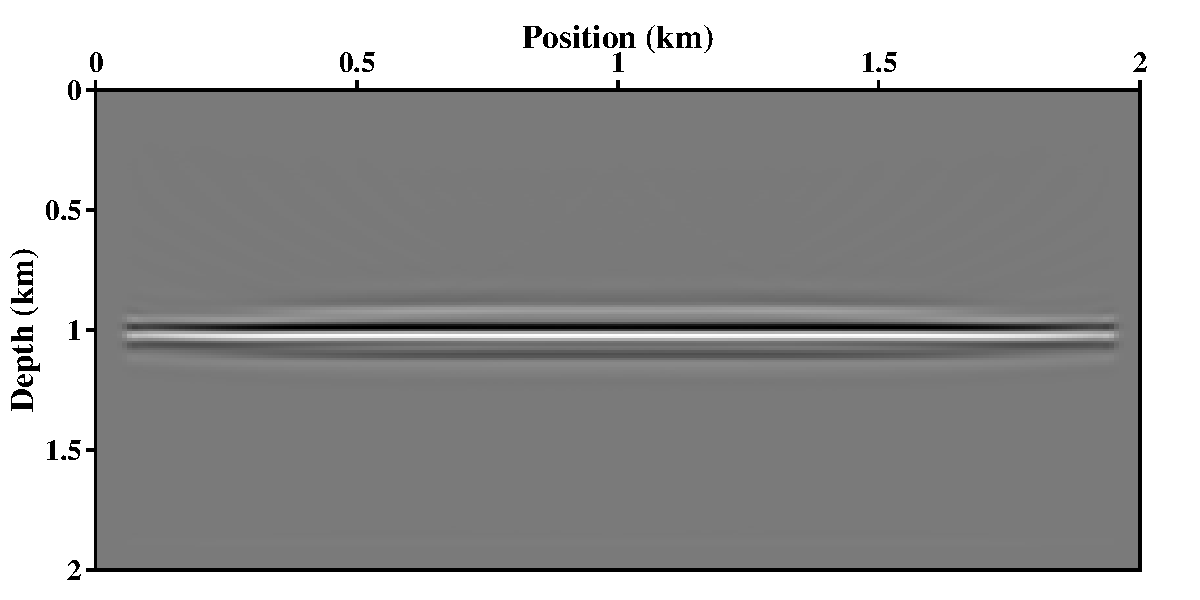
\includegraphics[width=0.48\textwidth]{Figure/chapter04/singlelayer/ref.pdf}}
   \caption{Sigbee2A model example. On the top are true models of 
   $V_p$ (a) and $V_s$ (b). On the bottom are initial models of $V_p$ (c) and $V_s$
   (d) linearly increasing with depth. }
   \label{fig:TrueAndInitial_1}
\end{figure}
\begin{figure}
   \centering
   \subfloat{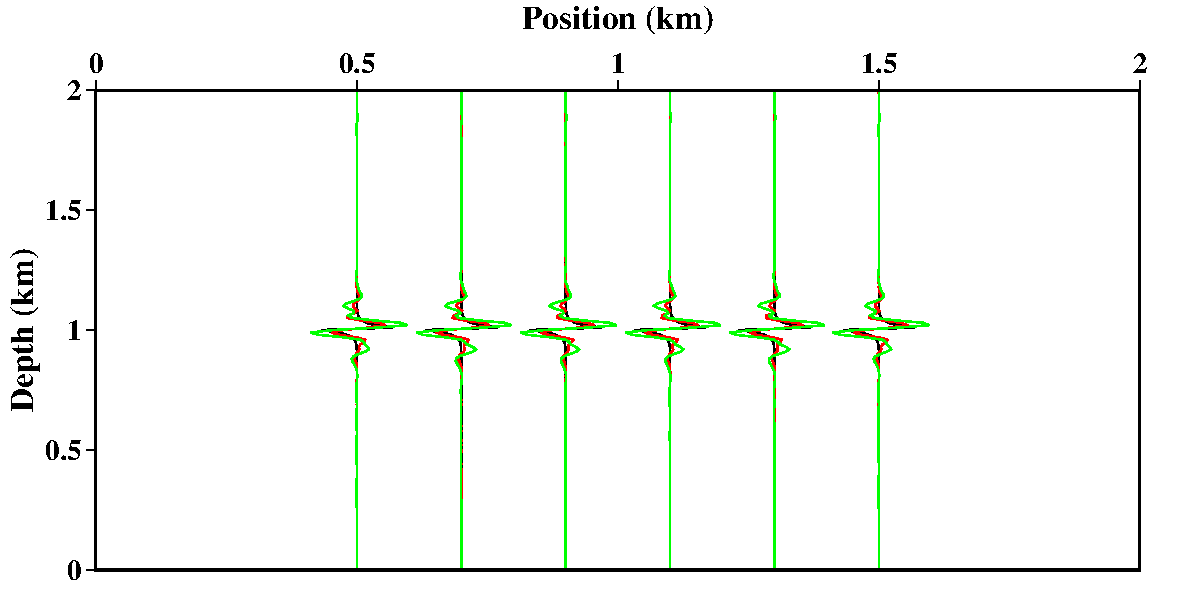
\includegraphics[width=0.58\textwidth]{Figure/chapter04/singlelayer/comparison.pdf}}\\
   \caption{Sigbee2A model example. On the top are true models of 
   $V_p$ (a) and $V_s$ (b). On the bottom are initial models of $V_p$ (c) and $V_s$
   (d) linearly increasing with depth. }
   \label{fig:line_comparison}
\end{figure}
\subsection{参数耦合的影响}
\begin{figure}
   \centering
   \subfloat[]{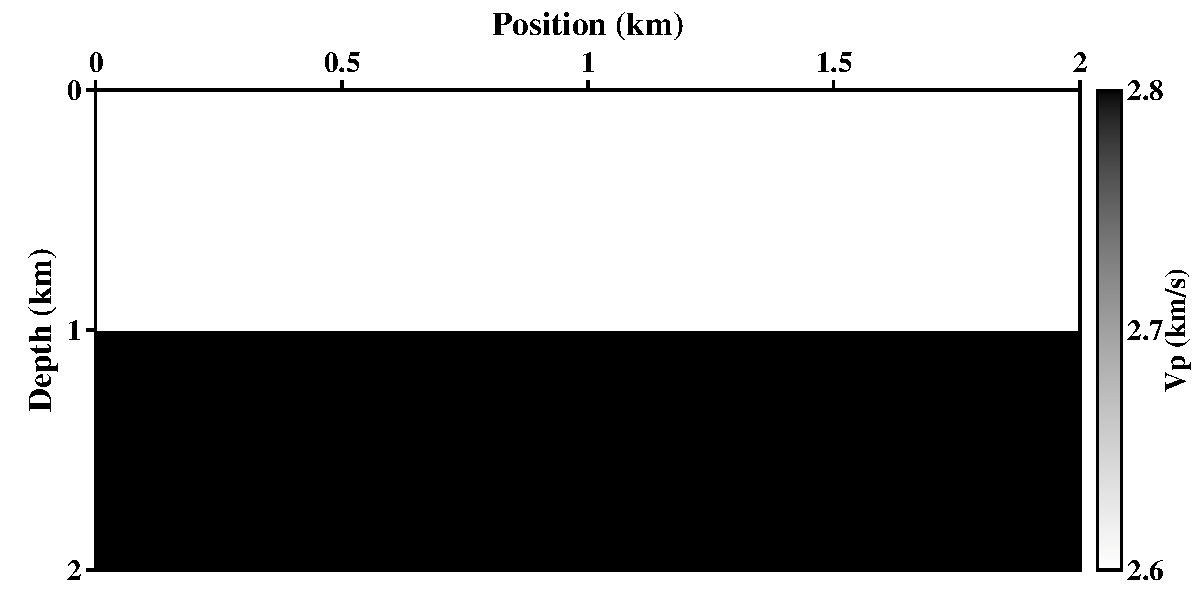
\includegraphics[width=0.48\textwidth]{Figure/chapter04/tradeoff/vp.pdf}}
   \subfloat[]{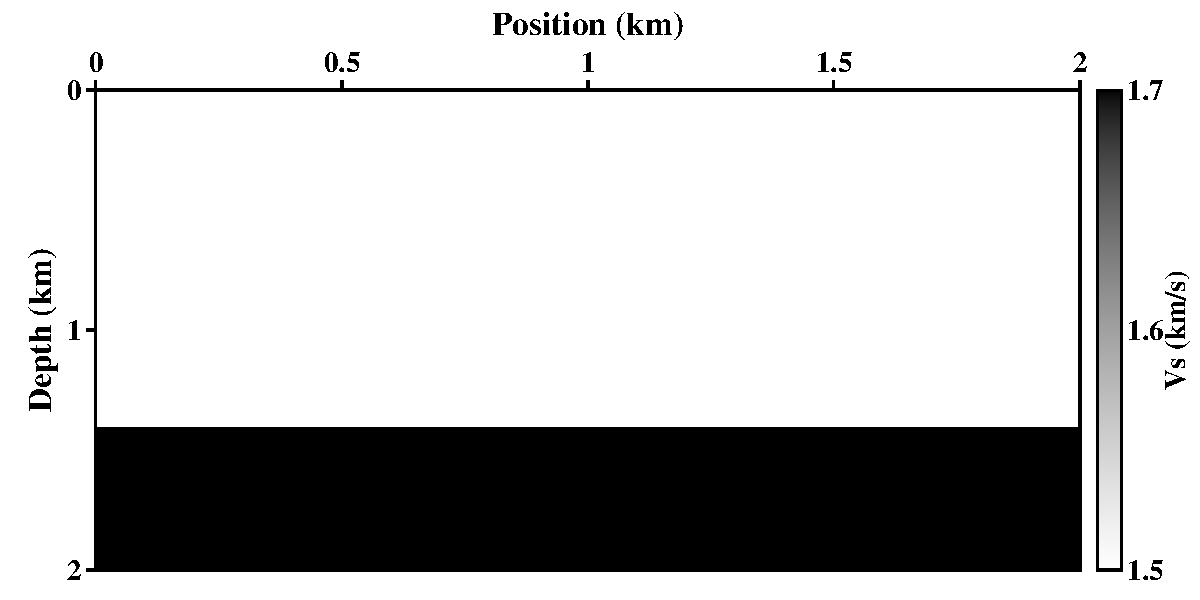
\includegraphics[width=0.48\textwidth]{Figure/chapter04/tradeoff/vs.pdf}}\\
   \subfloat[]{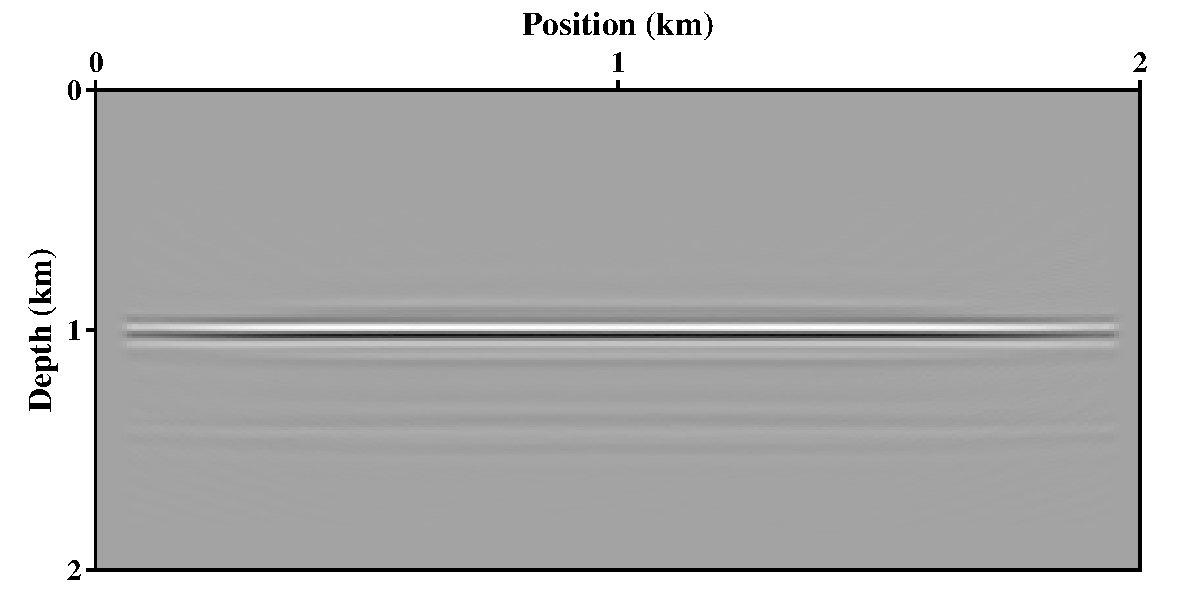
\includegraphics[width=0.48\textwidth]{Figure/chapter04/tradeoff/vpdecomp.pdf}}
   \subfloat[]{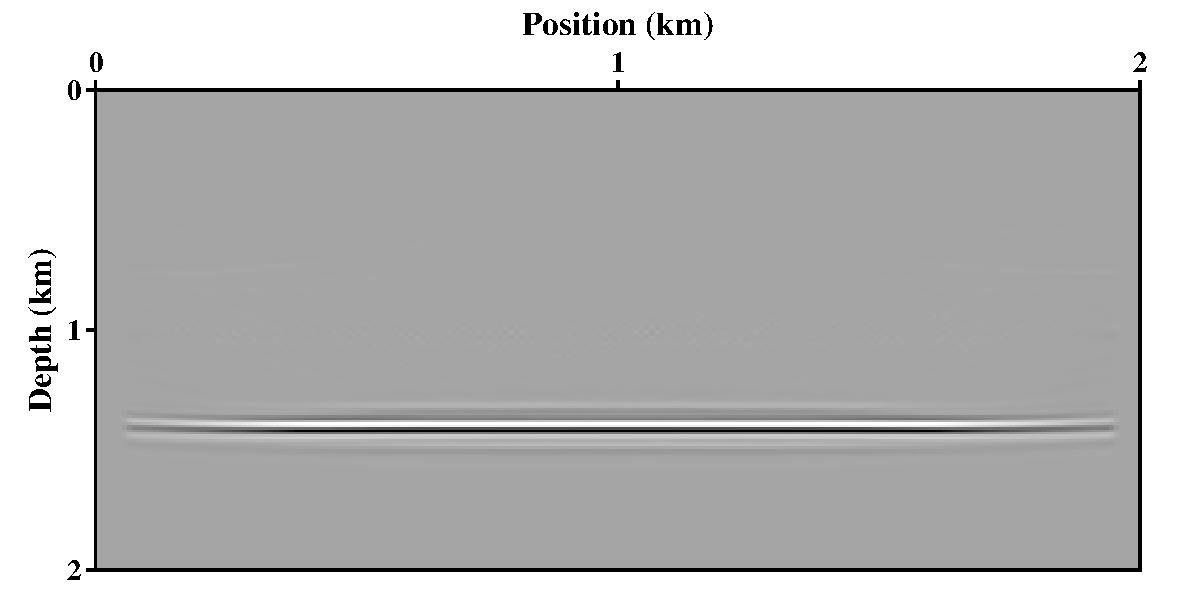
\includegraphics[width=0.48\textwidth]{Figure/chapter04/tradeoff/vsdecomp.pdf}}\\
   \subfloat[]{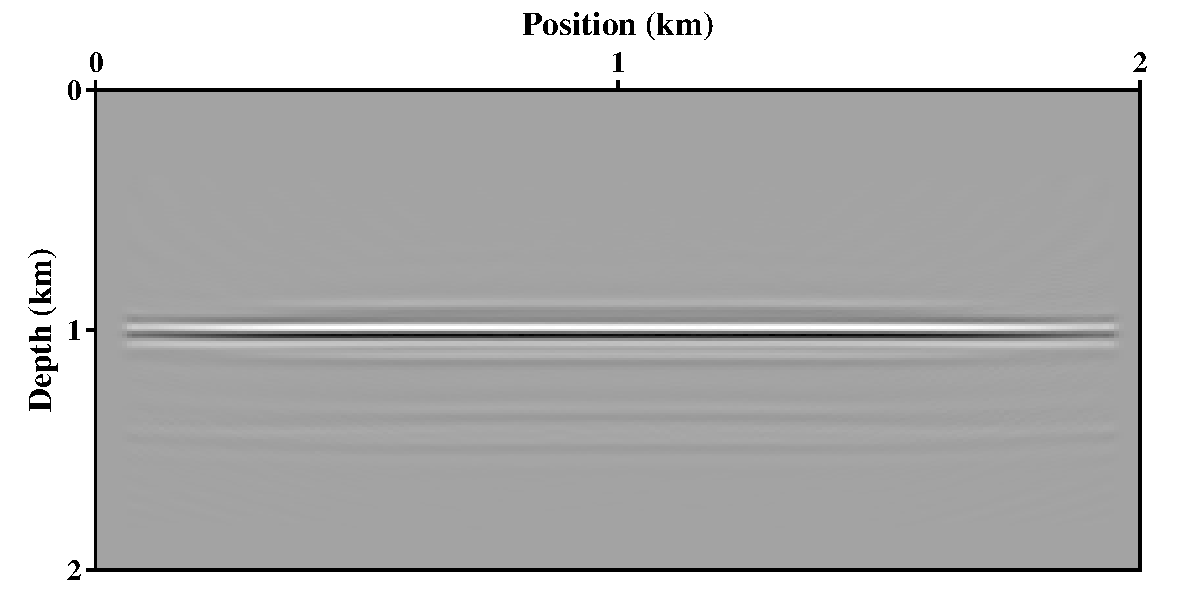
\includegraphics[width=0.48\textwidth]{Figure/chapter04/tradeoff/vpnodecomp.pdf}}
   \subfloat[]{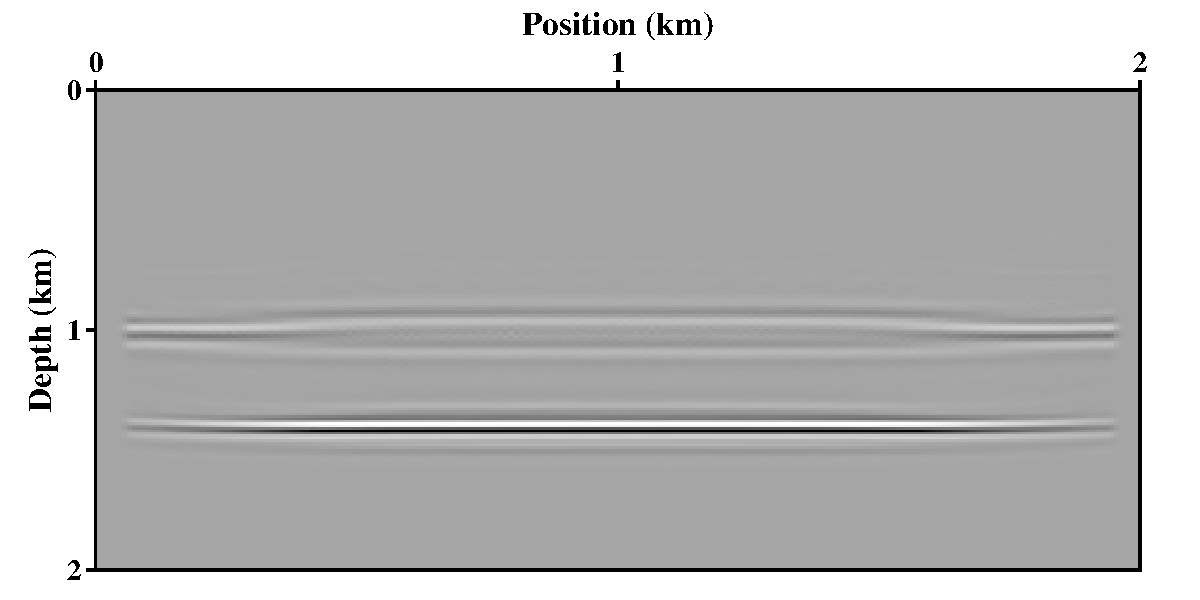
\includegraphics[width=0.48\textwidth]{Figure/chapter04/tradeoff/vsnodecomp.pdf}}
   \caption{Sigbee2A model example. On the top are true models of 
   $V_p$ (a) and $V_s$ (b). On the bottom are initial models of $V_p$ (c) and $V_s$
   (d) linearly increasing with depth. }
   \label{fig:tradeoff}
\end{figure}
\subsection{Marmousi模型}
\begin{figure}
   \centering
   \subfloat[]{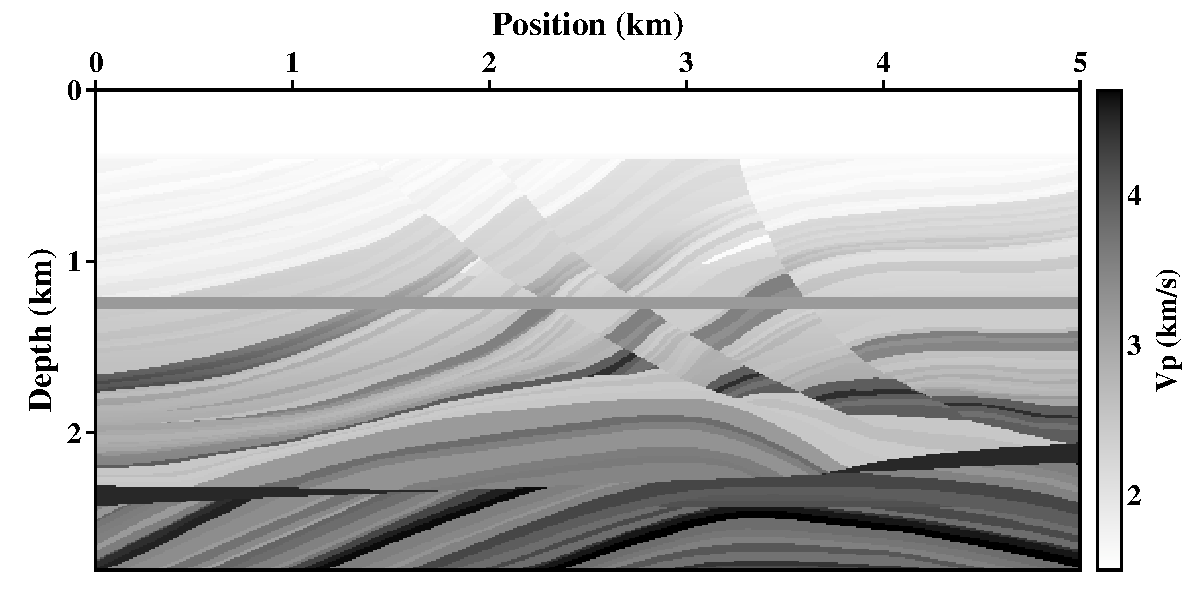
\includegraphics[width=0.48\textwidth]{Figure/chapter04/Marmousi/born/vp.pdf}}
   \subfloat[]{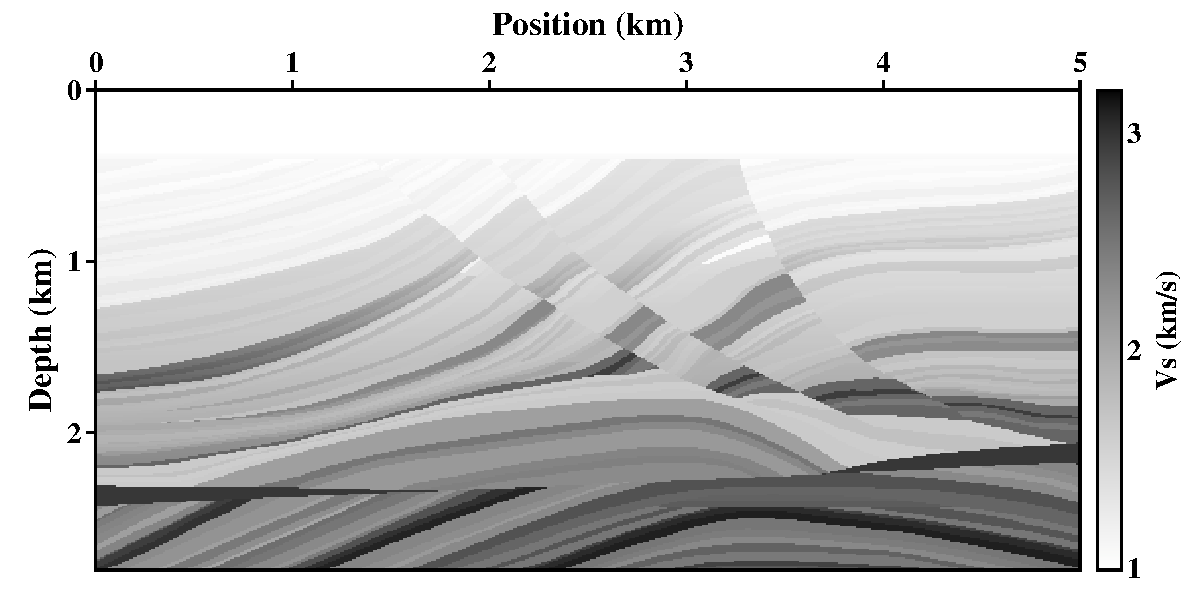
\includegraphics[width=0.48\textwidth]{Figure/chapter04/Marmousi/born/vs.pdf}}\\
   \subfloat[]{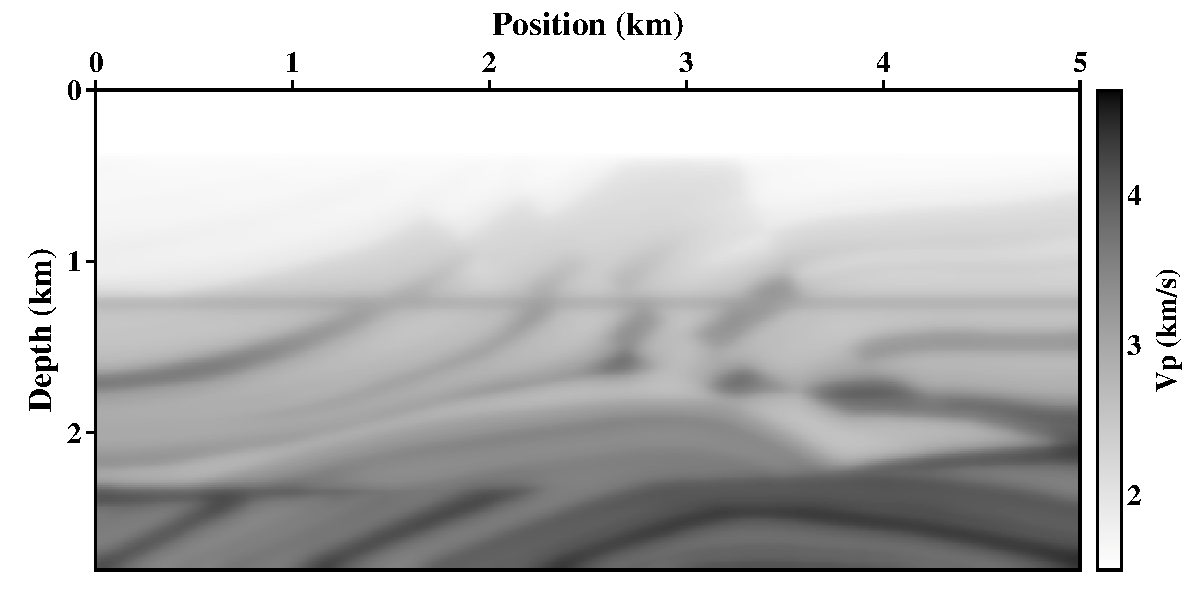
\includegraphics[width=0.48\textwidth]{Figure/chapter04/Marmousi/born/vpsmooth.pdf}}
   \subfloat[]{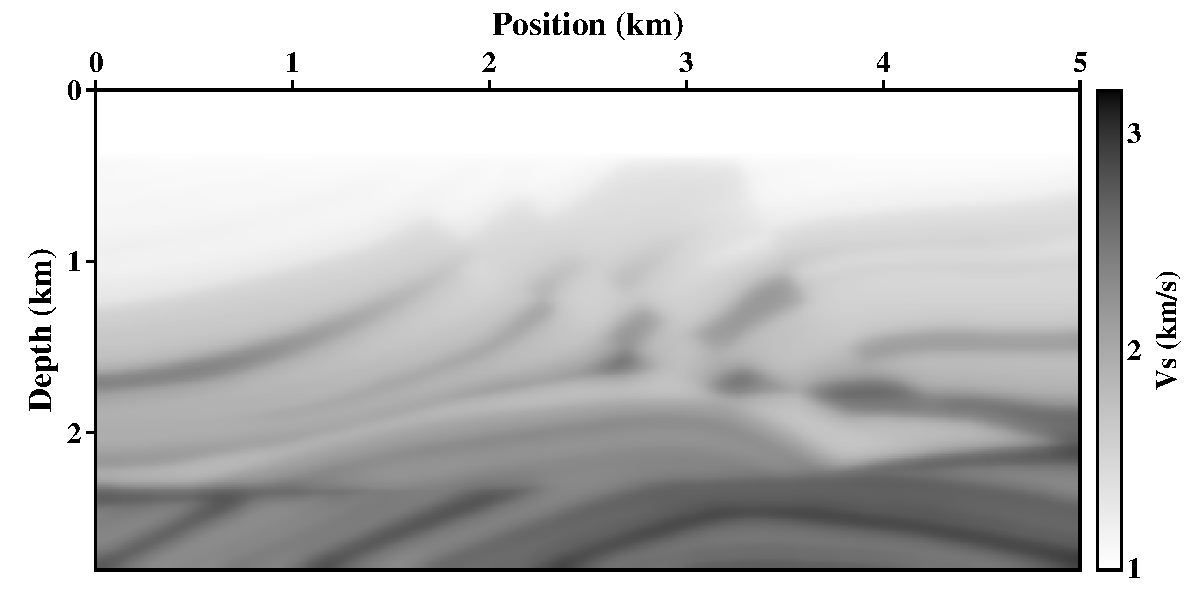
\includegraphics[width=0.48\textwidth]{Figure/chapter04/Marmousi/born/vssmooth.pdf}}
   \caption{Sigbee2A model example. On the top are true models of 
   $V_p$ (a) and $V_s$ (b). On the bottom are initial models of $V_p$ (c) and $V_s$
   (d) linearly increasing with depth. }
   \label{fig:TrueAndInitial_1}
\end{figure}
\begin{figure}
   \centering
   \subfloat[]{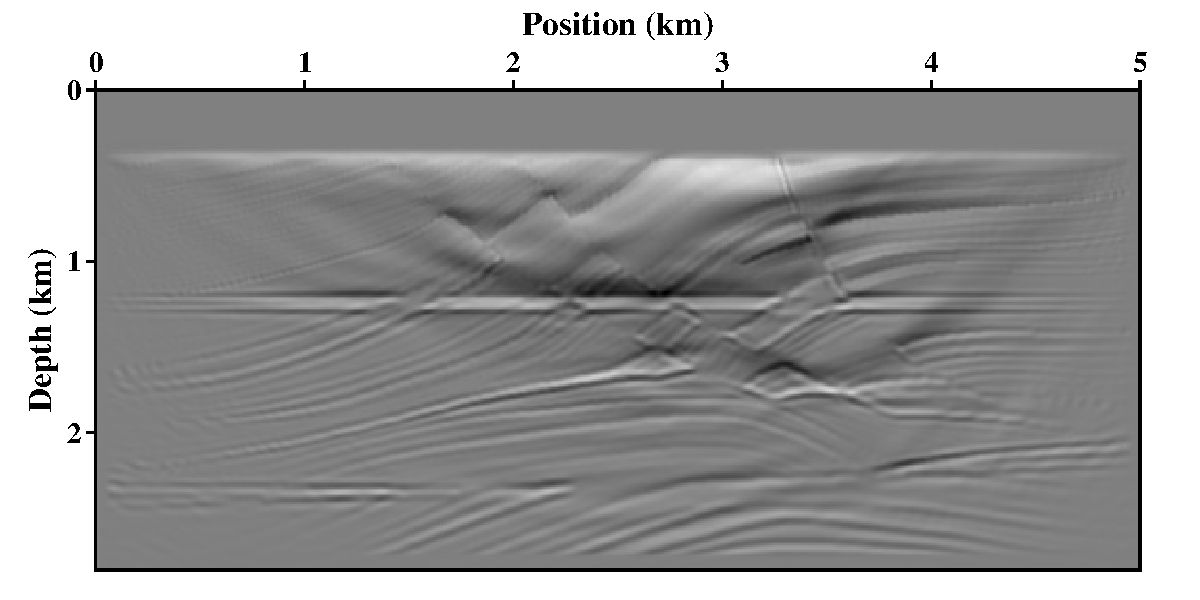
\includegraphics[width=0.48\textwidth]{Figure/chapter04/Marmousi/born/RTMvpdecomp.pdf}}
   \subfloat[]{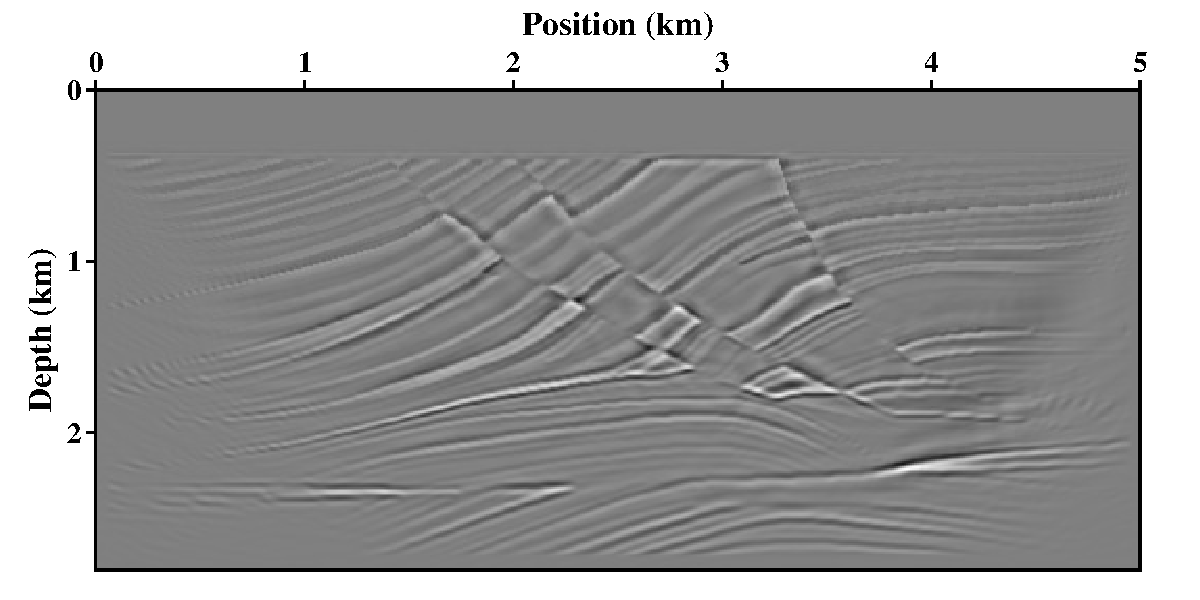
\includegraphics[width=0.48\textwidth]{Figure/chapter04/Marmousi/born/RTMvsdecomp.pdf}}\\
   \subfloat[]{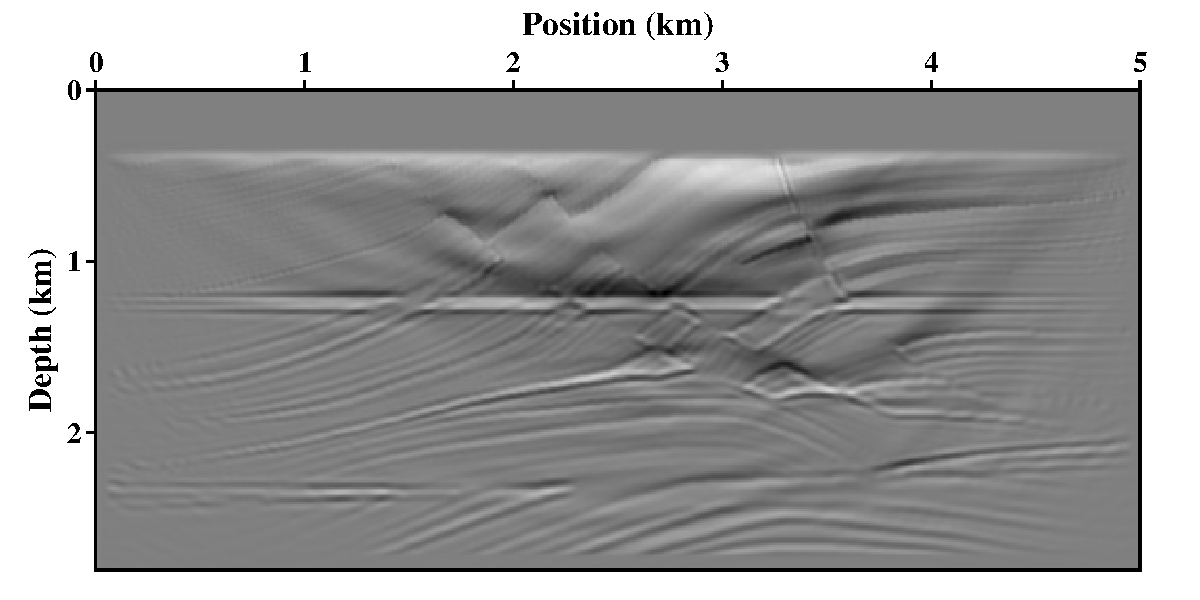
\includegraphics[width=0.48\textwidth]{Figure/chapter04/Marmousi/born/RTMvpnodecomp.pdf}}
   \subfloat[]{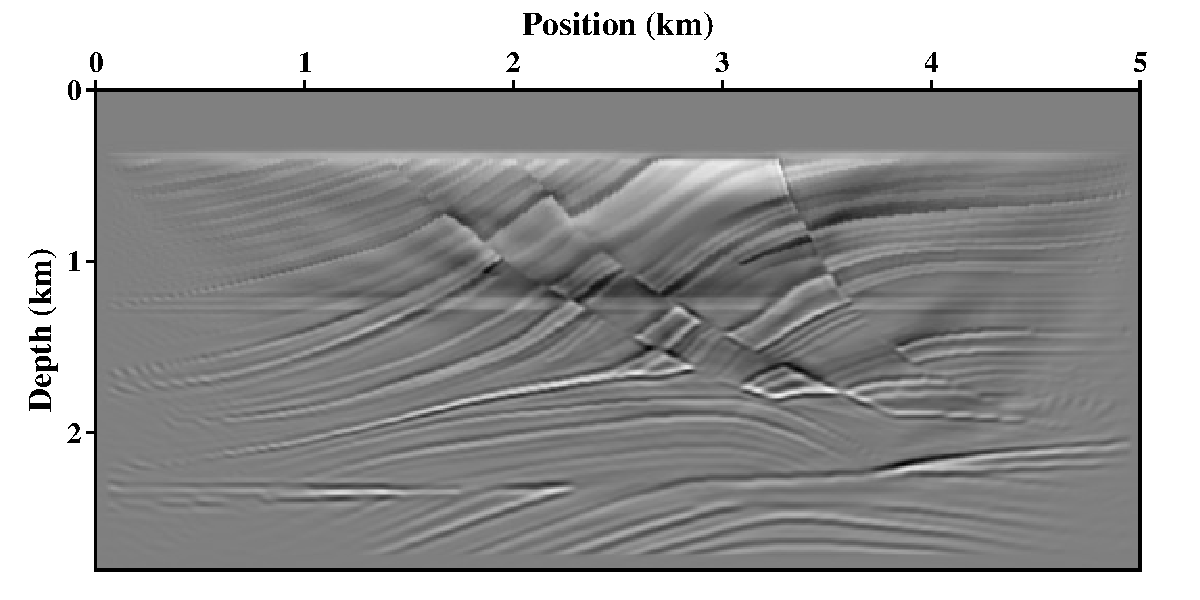
\includegraphics[width=0.48\textwidth]{Figure/chapter04/Marmousi/born/RTMvsnodecomp.pdf}}
   \caption{Sigbee2A model example. On the top are true models of 
   $V_p$ (a) and $V_s$ (b). On the bottom are initial models of $V_p$ (c) and $V_s$
   (d) linearly increasing with depth. }
   \label{fig:RTM_1}
\end{figure}
\begin{figure}
   \centering
   \subfloat[]{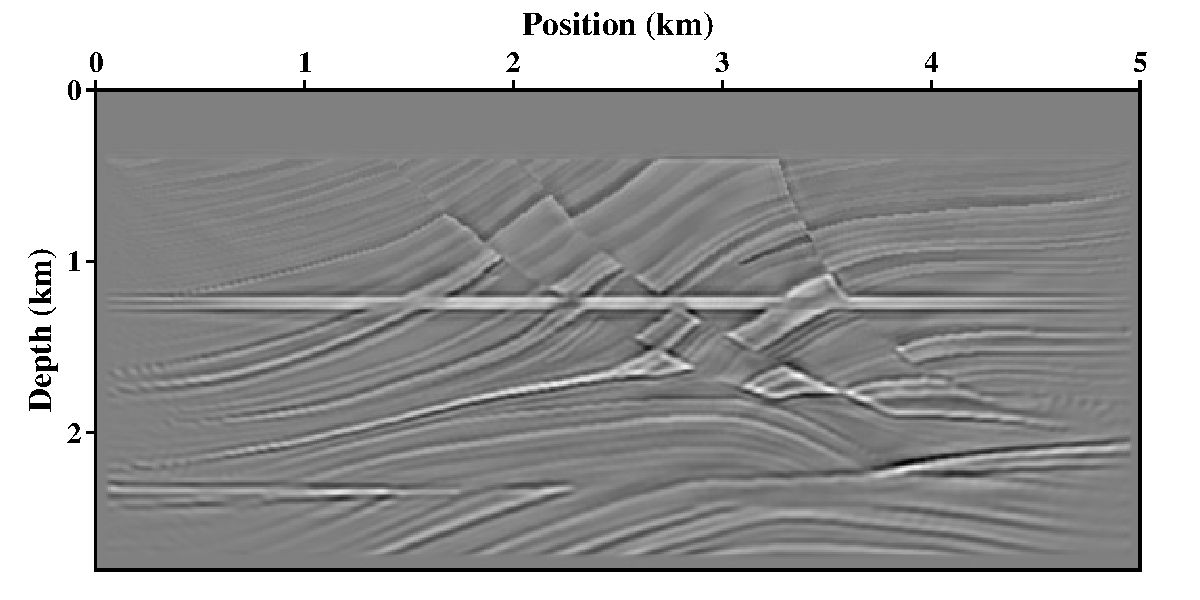
\includegraphics[width=0.48\textwidth]{Figure/chapter04/Marmousi/born/vpdecomp.pdf}}
   \subfloat[]{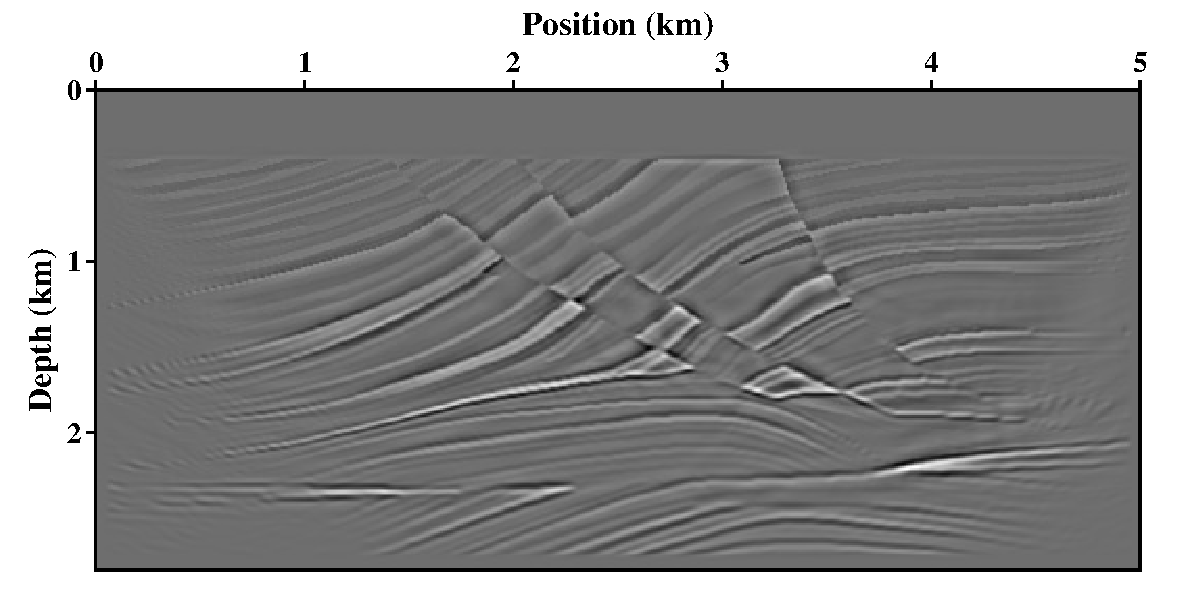
\includegraphics[width=0.48\textwidth]{Figure/chapter04/Marmousi/born/vsdecomp.pdf}}\\
   \subfloat[]{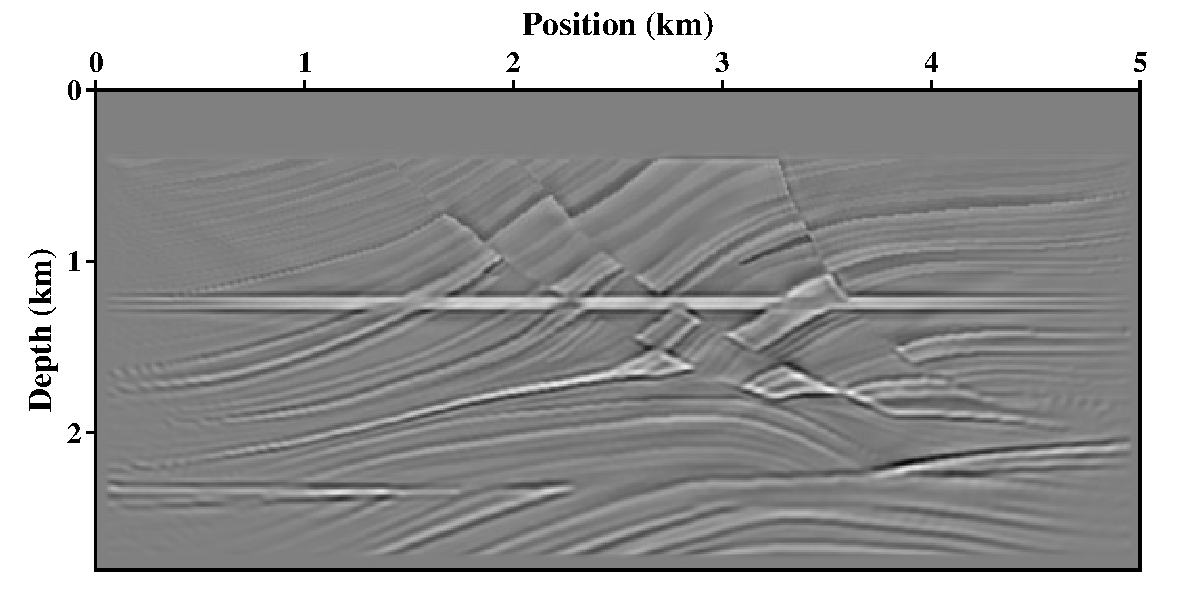
\includegraphics[width=0.48\textwidth]{Figure/chapter04/Marmousi/born/vpnodecomp.pdf}}
   \subfloat[]{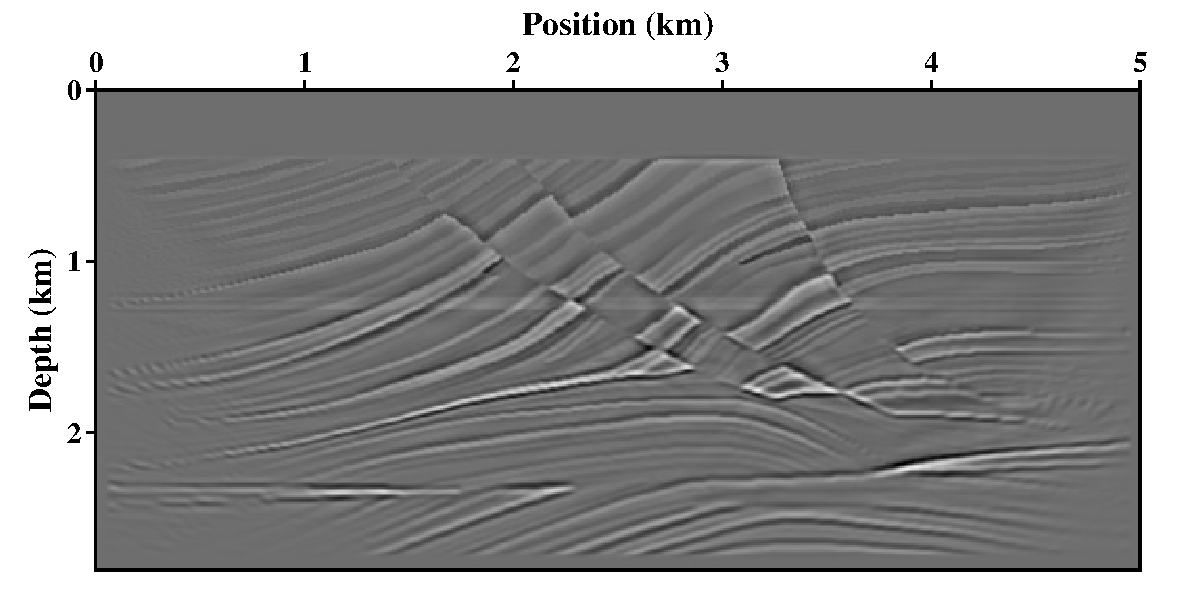
\includegraphics[width=0.48\textwidth]{Figure/chapter04/Marmousi/born/vsnodecomp.pdf}}
   \caption{Sigbee2A model example. On the top are true models of 
   $V_p$ (a) and $V_s$ (b). On the bottom are initial models of $V_p$ (c) and $V_s$
   (d) linearly increasing with depth. }
   \label{fig:LSRTM_1}
\end{figure}
\begin{figure}
   \centering
   \subfloat[]{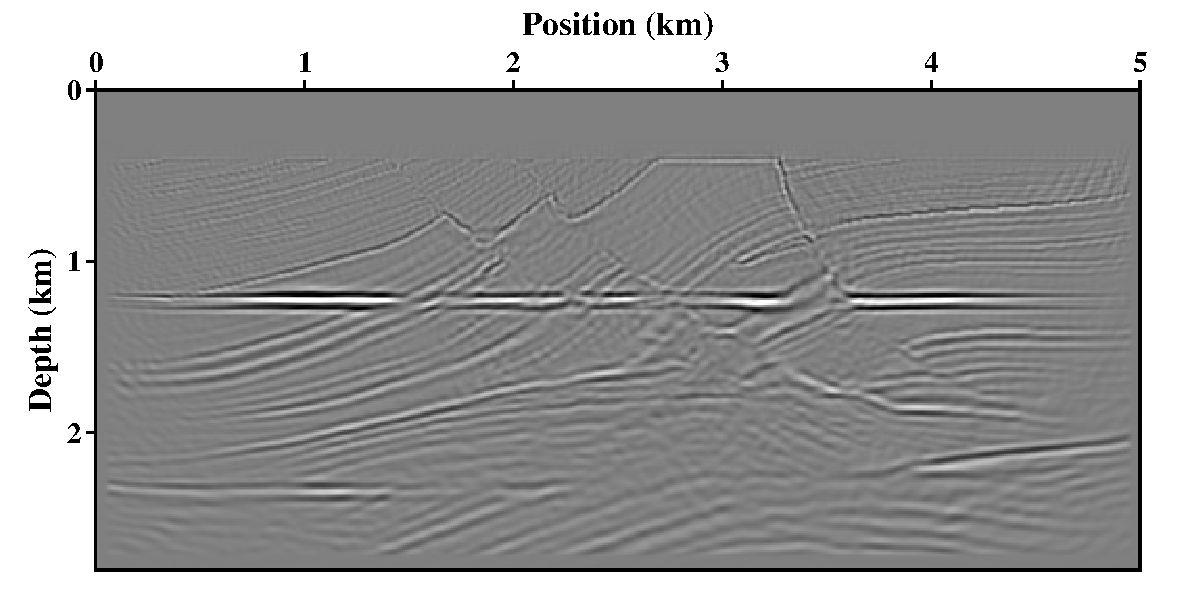
\includegraphics[width=0.48\textwidth]{Figure/chapter04/Marmousi/reflection/RTMvpdecomp.pdf}}
   \subfloat[]{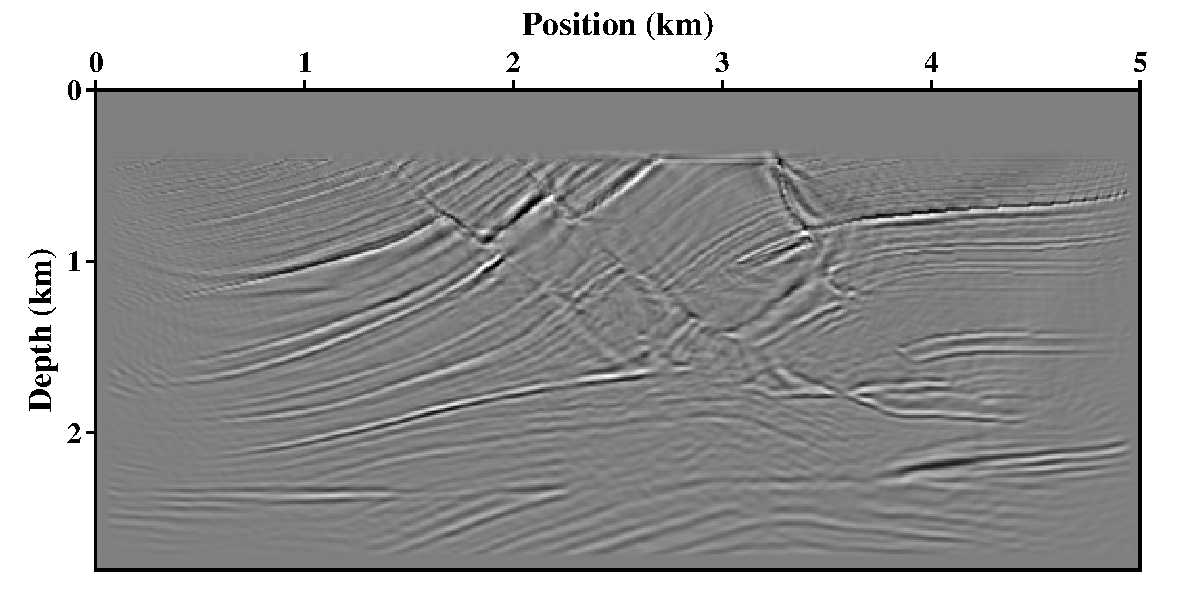
\includegraphics[width=0.48\textwidth]{Figure/chapter04/Marmousi/reflection/RTMvsdecomp.pdf}}\\
   \subfloat[]{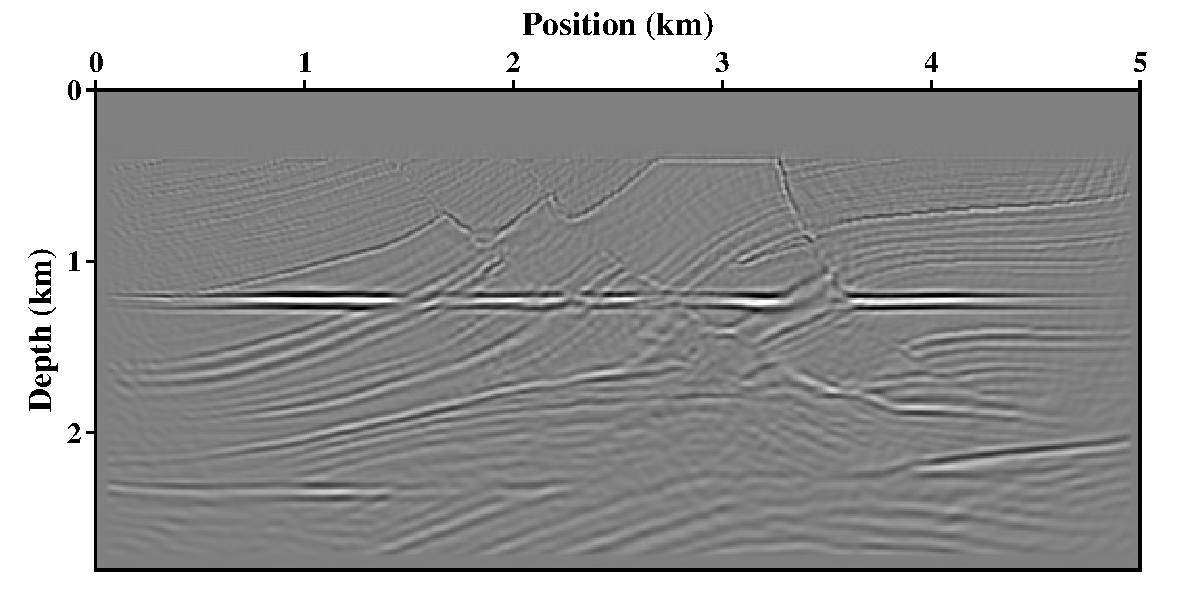
\includegraphics[width=0.48\textwidth]{Figure/chapter04/Marmousi/reflection/RTMvpnodecomp.pdf}}
   \subfloat[]{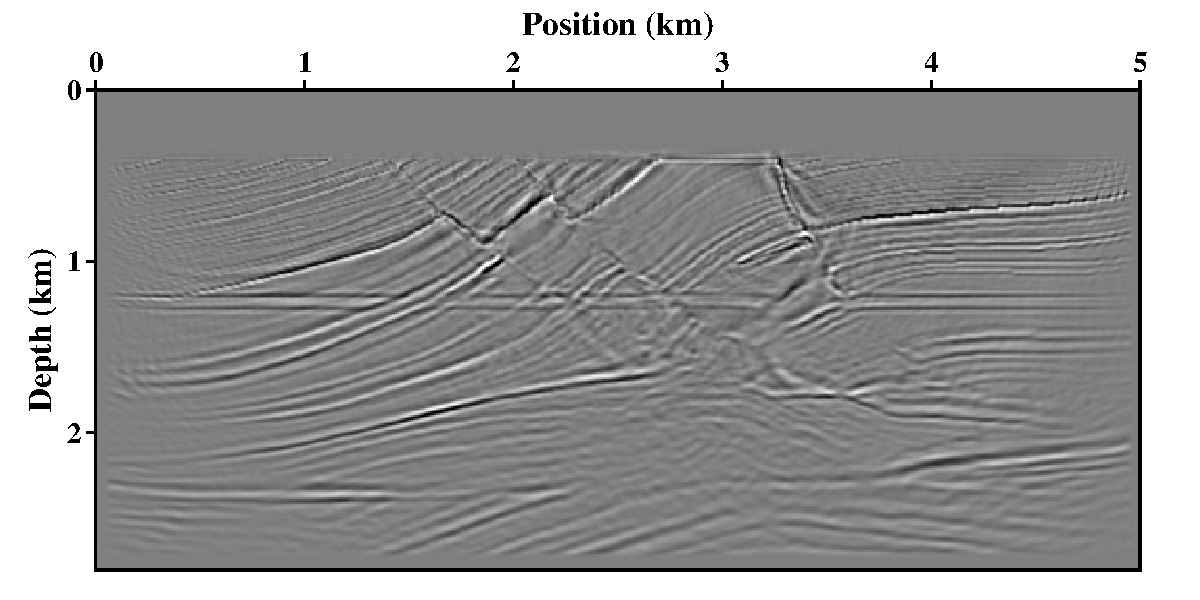
\includegraphics[width=0.48\textwidth]{Figure/chapter04/Marmousi/reflection/RTMvsnodecomp.pdf}}
   \caption{Sigbee2A model example. On the top are true models of 
   $V_p$ (a) and $V_s$ (b). On the bottom are initial models of $V_p$ (c) and $V_s$
   (d) linearly increasing with depth. }
   \label{fig:RTM_1_refl}
\end{figure}
\begin{figure}
   \centering
   \subfloat[]{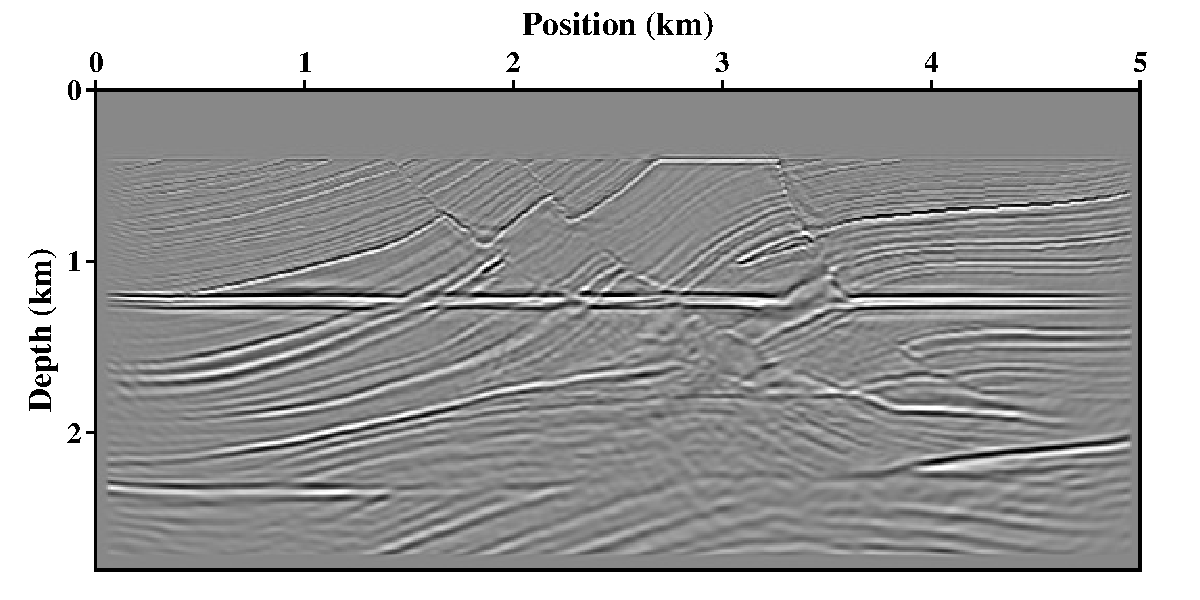
\includegraphics[width=0.48\textwidth]{Figure/chapter04/Marmousi/reflection/vpdecomp.pdf}}
   \subfloat[]{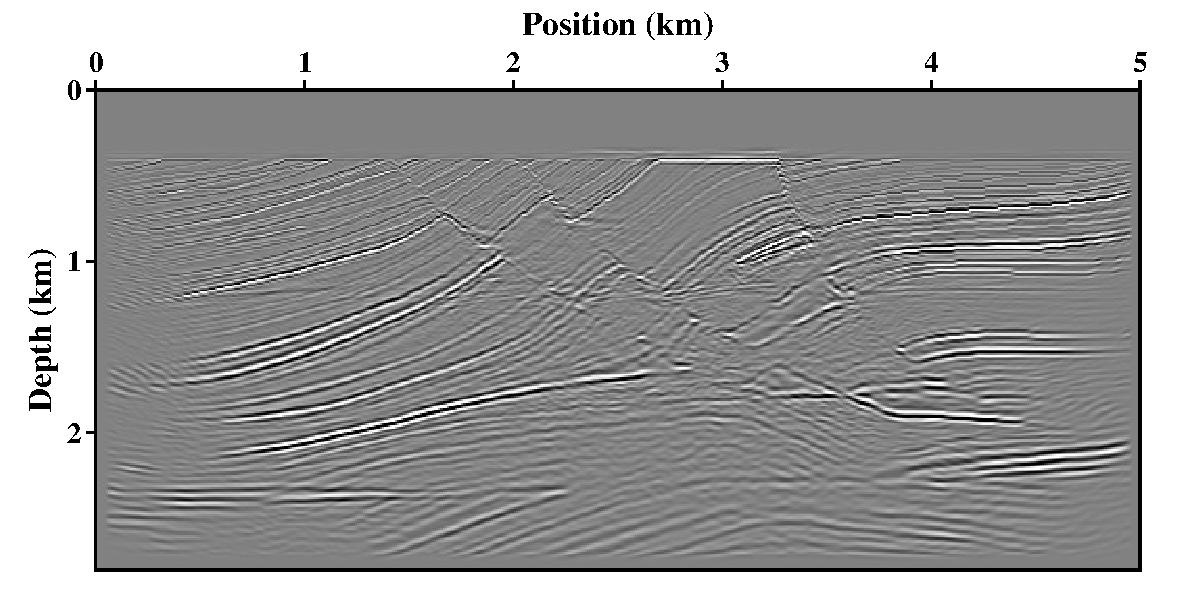
\includegraphics[width=0.48\textwidth]{Figure/chapter04/Marmousi/reflection/vsdecomp.pdf}}\\
   \subfloat[]{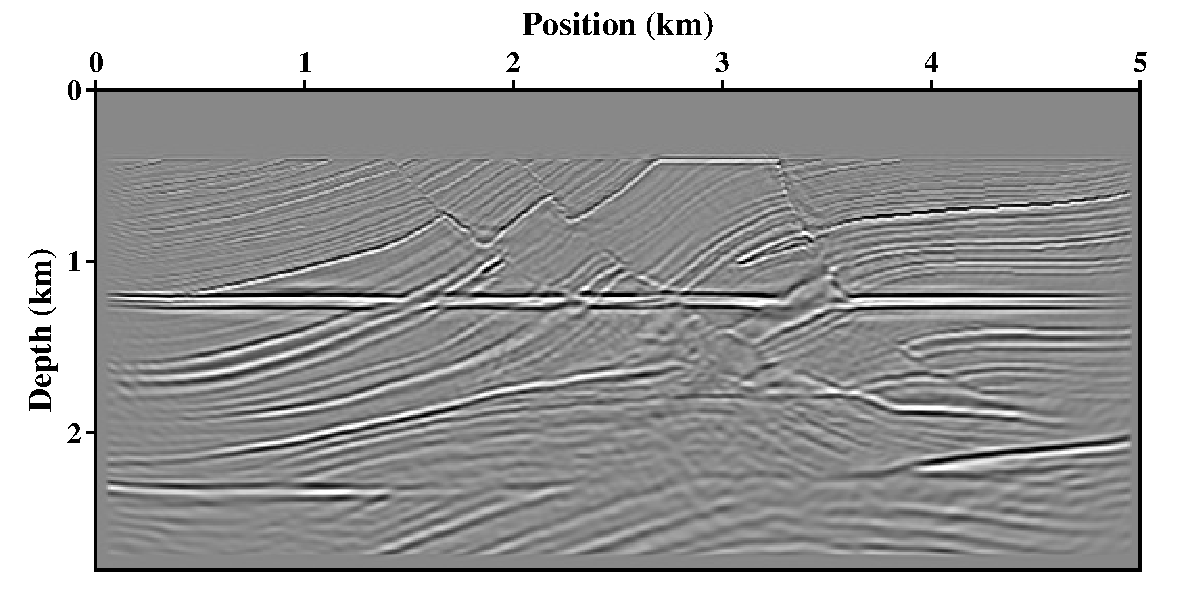
\includegraphics[width=0.48\textwidth]{Figure/chapter04/Marmousi/reflection/vpnodecomp.pdf}}
   \subfloat[]{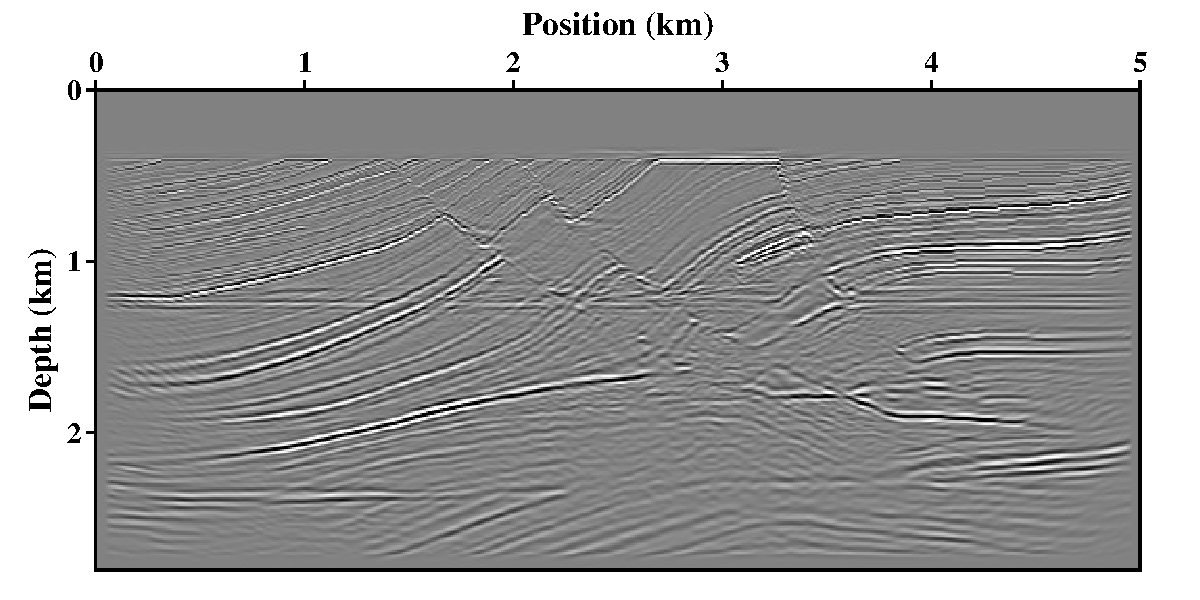
\includegraphics[width=0.48\textwidth]{Figure/chapter04/Marmousi/reflection/vsnodecomp.pdf}}
   \caption{Sigbee2A model example. On the top are true models of 
   $V_p$ (a) and $V_s$ (b). On the bottom are initial models of $V_p$ (c) and $V_s$
   (d) linearly increasing with depth. }
   \label{fig:LSRTM_1_refl}
\end{figure}
\begin{figure}
   \centering
   \subfloat[]{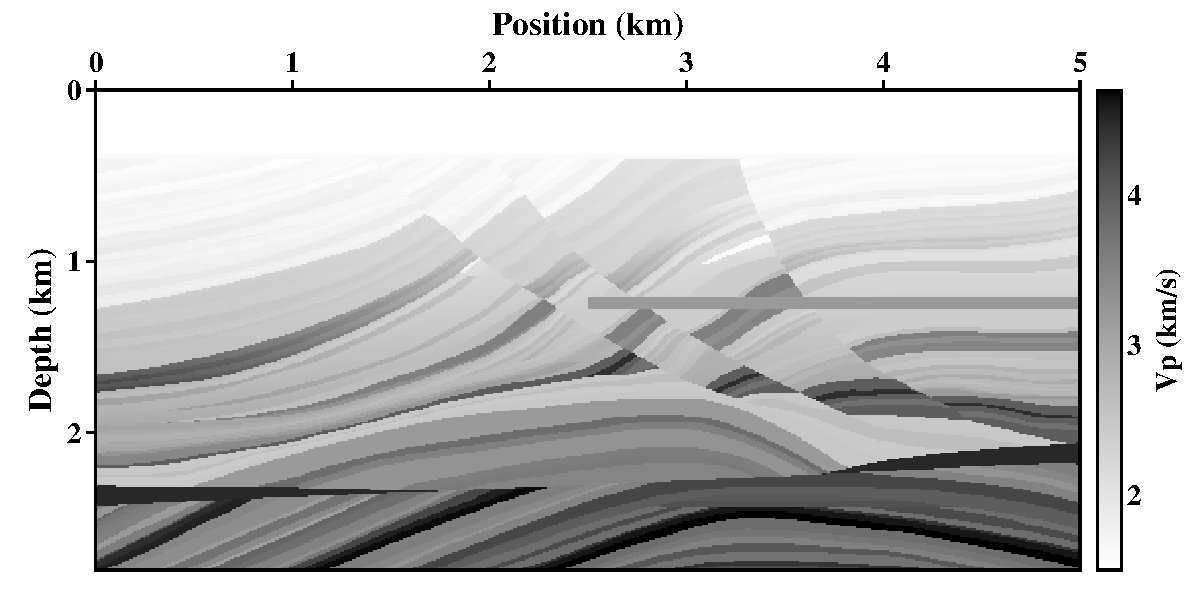
\includegraphics[width=0.48\textwidth]{Figure/chapter04/Marmousi/Vsborn/vp.pdf}}
   \subfloat[]{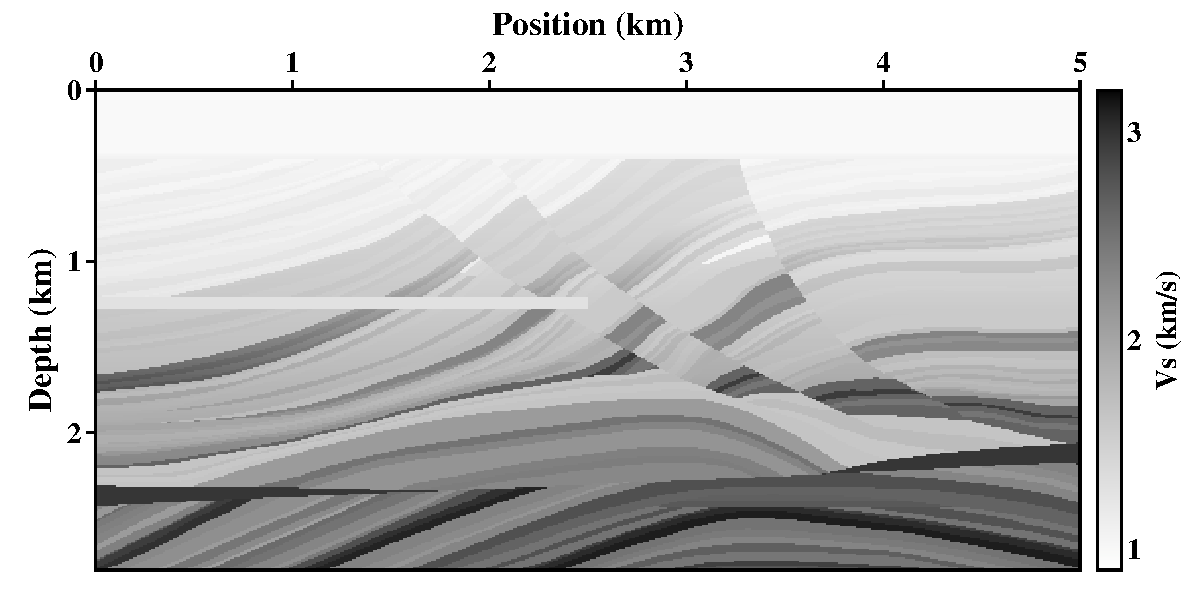
\includegraphics[width=0.48\textwidth]{Figure/chapter04/Marmousi/Vsborn/vs.pdf}}\\
   \subfloat[]{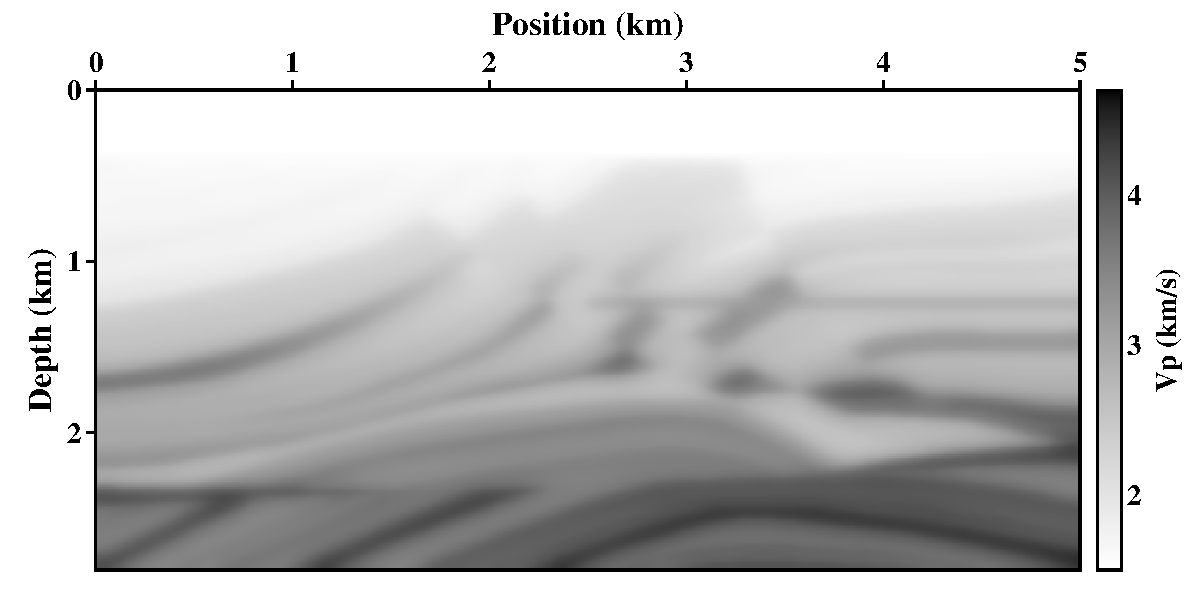
\includegraphics[width=0.48\textwidth]{Figure/chapter04/Marmousi/Vsborn/vpsmooth.pdf}}
   \subfloat[]{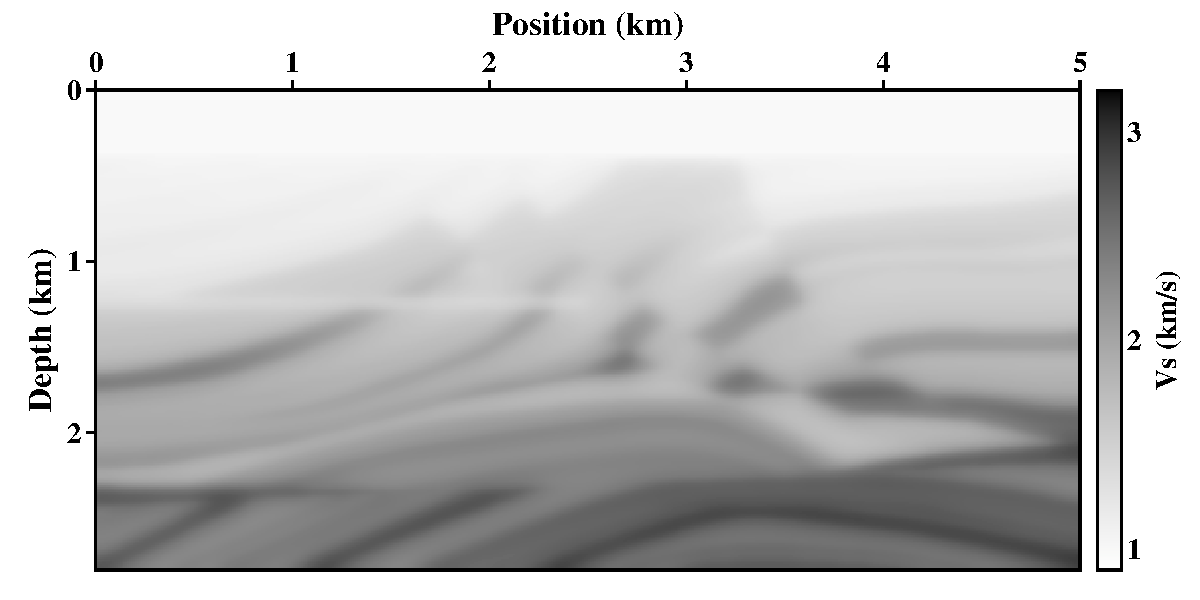
\includegraphics[width=0.48\textwidth]{Figure/chapter04/Marmousi/Vsborn/vssmooth.pdf}}
   \caption{Sigbee2A model example. On the top are true models of 
   $V_p$ (a) and $V_s$ (b). On the bottom are initial models of $V_p$ (c) and $V_s$
   (d) linearly increasing with depth. }
   \label{fig:TrueAndInitial_2}
\end{figure}
\begin{figure}
   \centering
   \subfloat[]{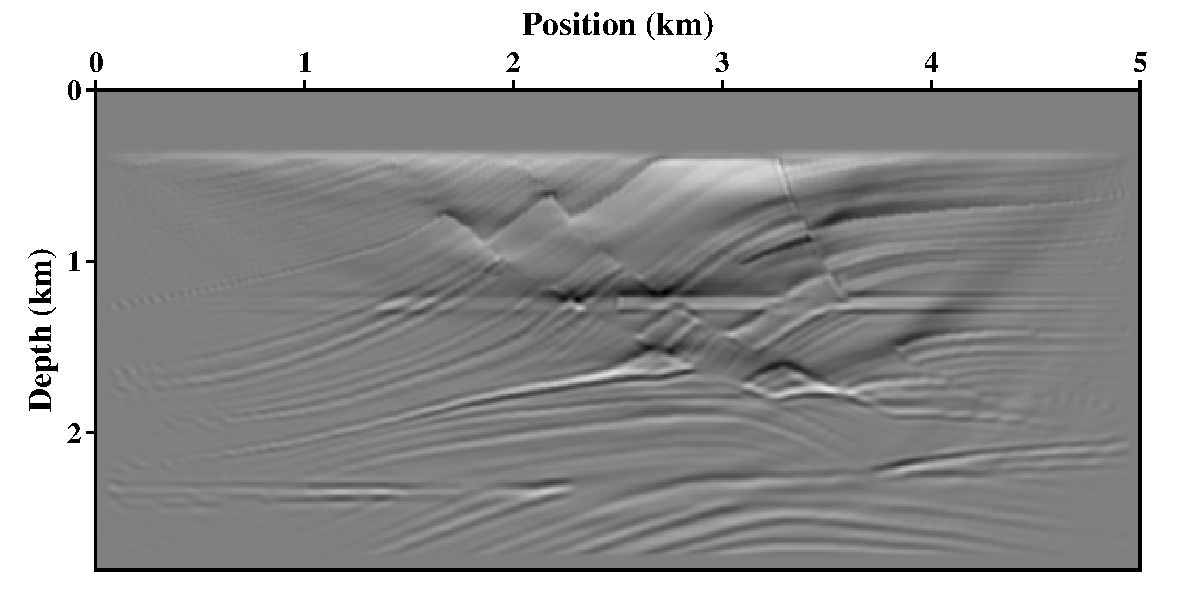
\includegraphics[width=0.48\textwidth]{Figure/chapter04/Marmousi/Vsborn/RTMvpdecomp.pdf}}
   \subfloat[]{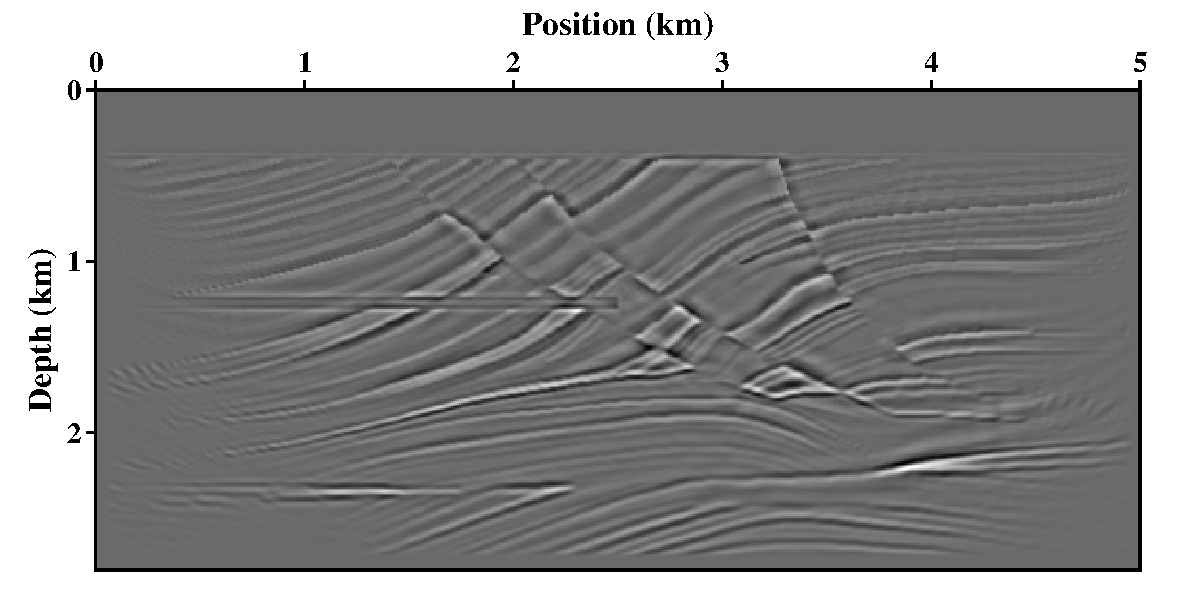
\includegraphics[width=0.48\textwidth]{Figure/chapter04/Marmousi/Vsborn/RTMvsdecomp.pdf}}\\
   \subfloat[]{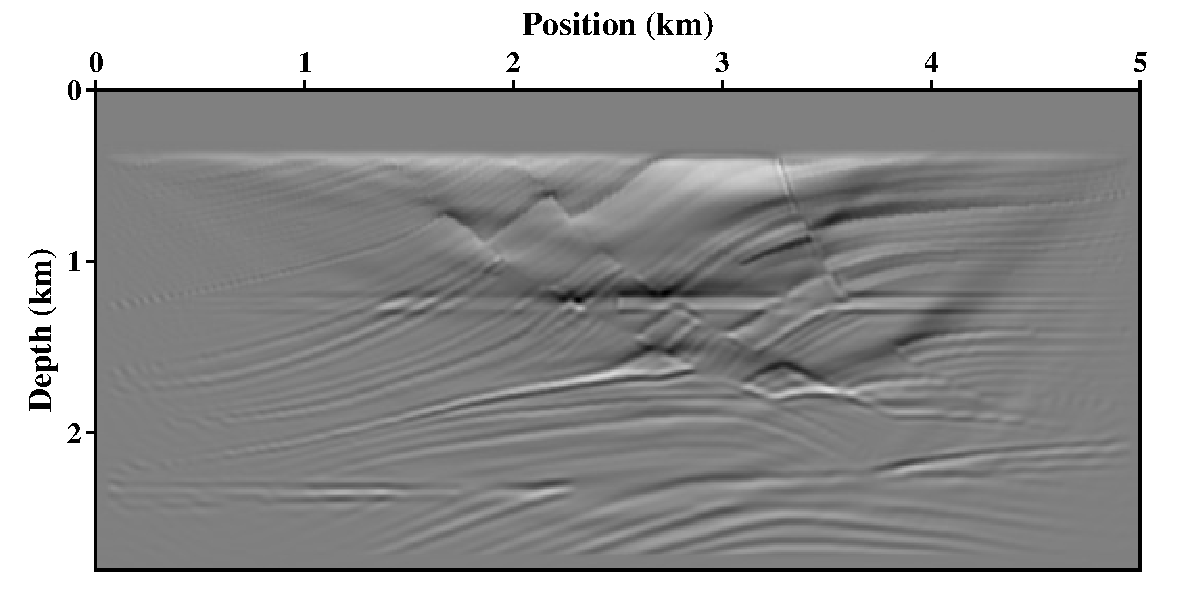
\includegraphics[width=0.48\textwidth]{Figure/chapter04/Marmousi/Vsborn/RTMvpnodecomp.pdf}}
   \subfloat[]{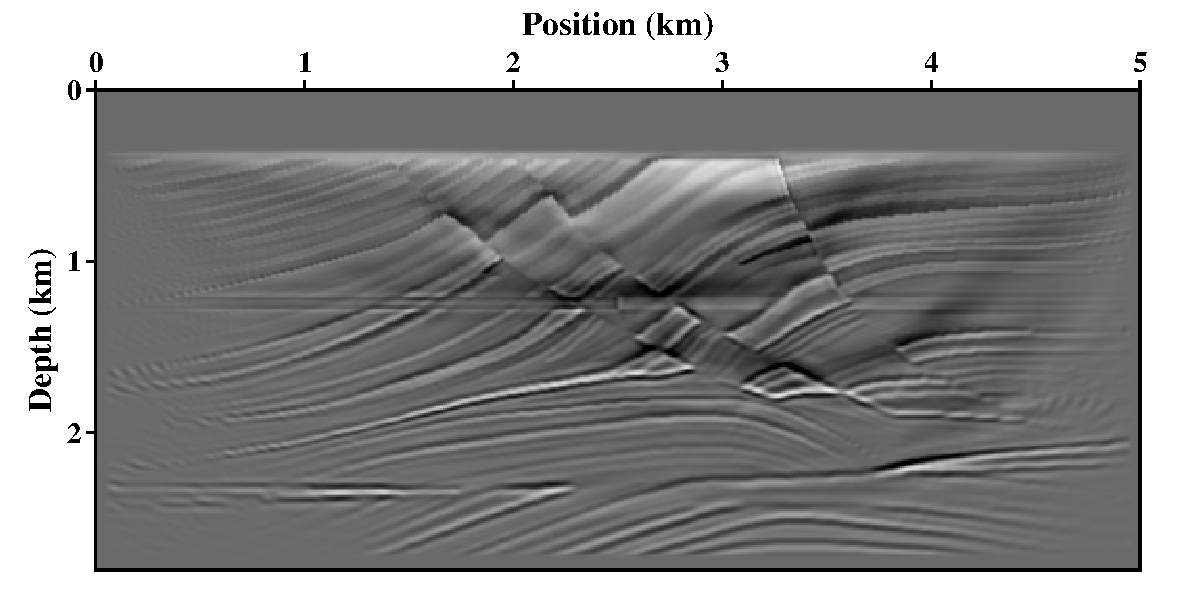
\includegraphics[width=0.48\textwidth]{Figure/chapter04/Marmousi/Vsborn/RTMvsnodecomp.pdf}}
   \caption{Sigbee2A model example. On the top are true models of 
   $V_p$ (a) and $V_s$ (b). On the bottom are initial models of $V_p$ (c) and $V_s$
   (d) linearly increasing with depth. }
   \label{fig:RTM_2}
\end{figure}
\begin{figure}
   \centering
   \subfloat[]{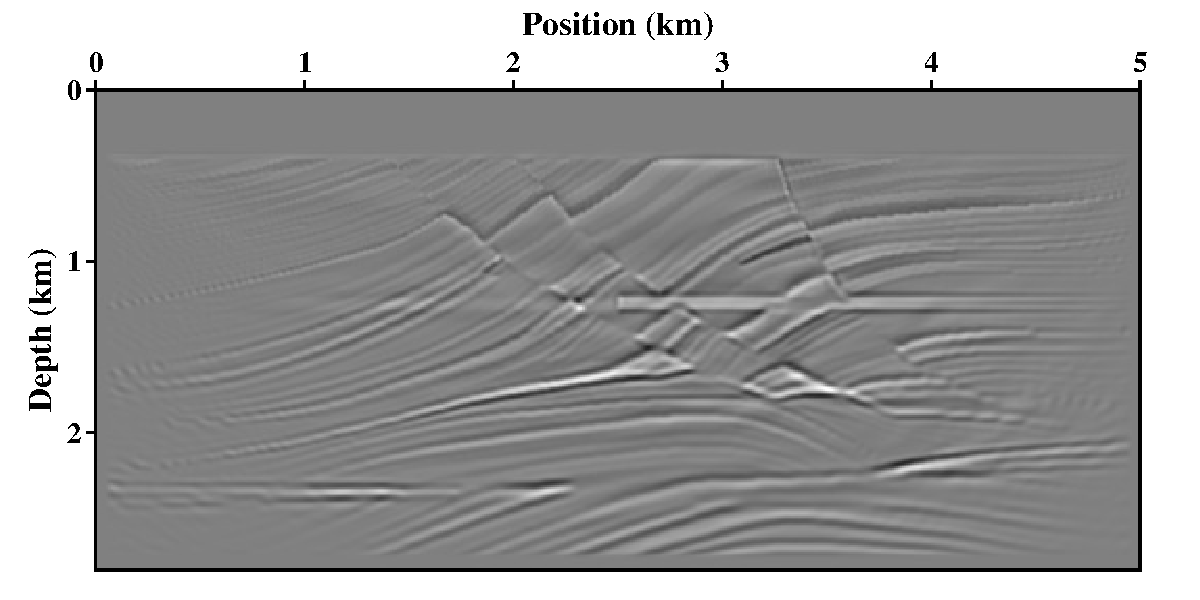
\includegraphics[width=0.48\textwidth]{Figure/chapter04/Marmousi/Vsborn/vpdecomp.pdf}}
   \subfloat[]{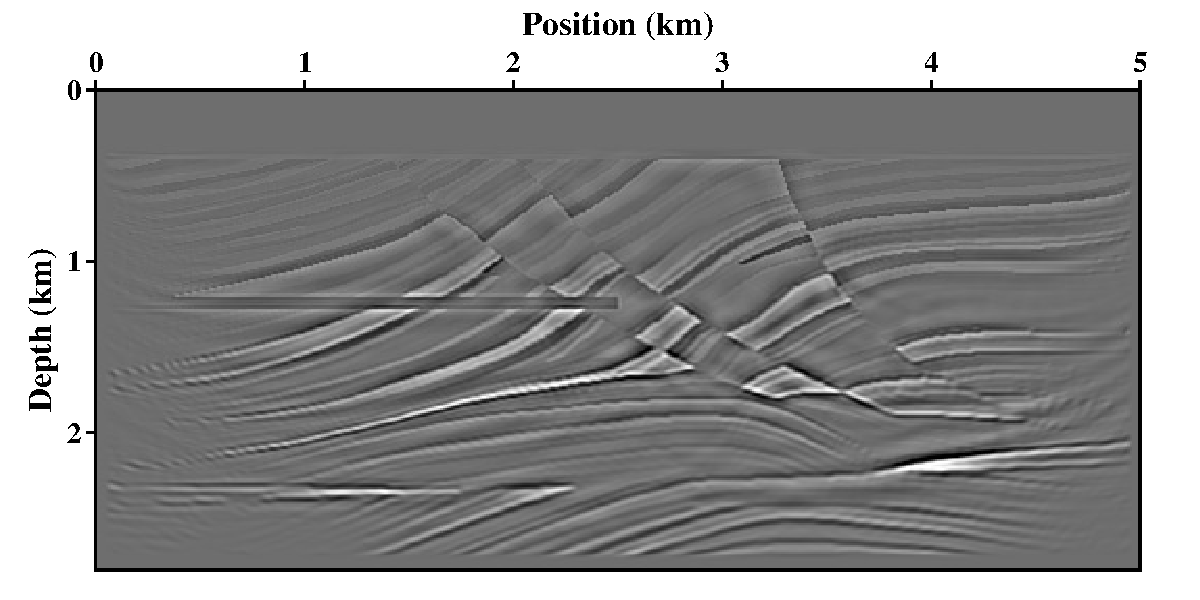
\includegraphics[width=0.48\textwidth]{Figure/chapter04/Marmousi/Vsborn/vsdecomp.pdf}}\\
   \subfloat[]{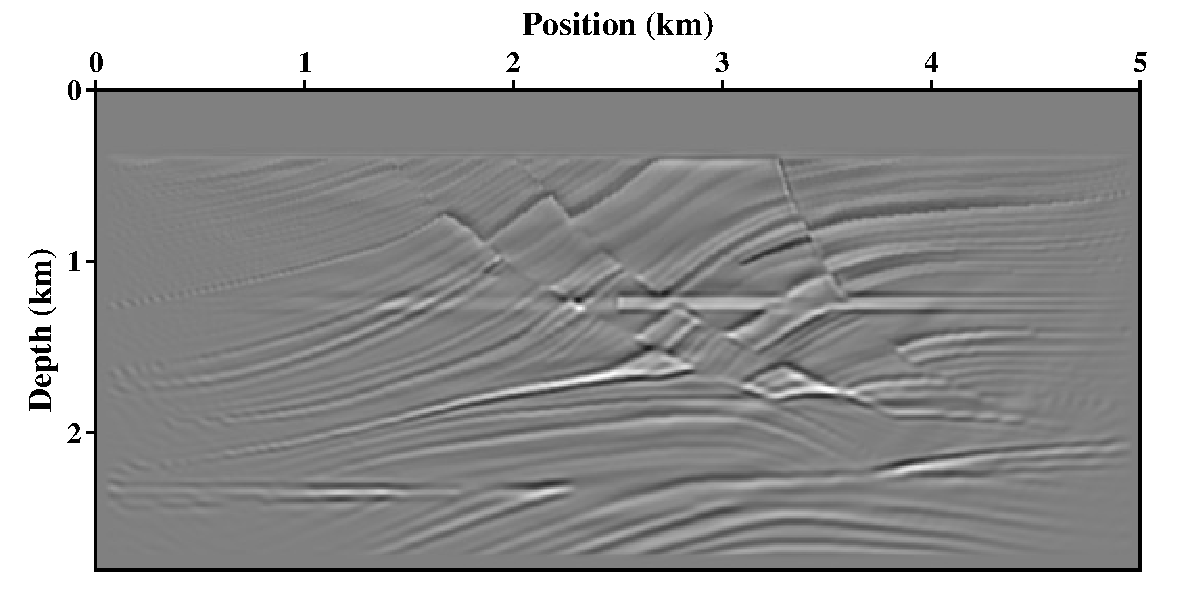
\includegraphics[width=0.48\textwidth]{Figure/chapter04/Marmousi/Vsborn/vpnodecomp.pdf}}
   \subfloat[]{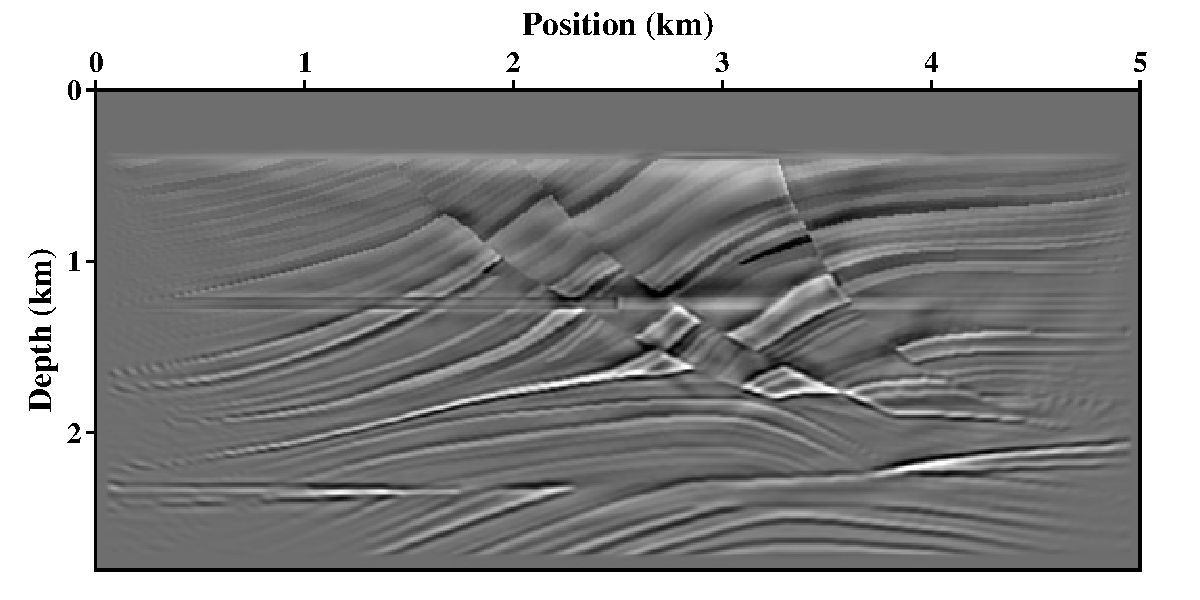
\includegraphics[width=0.48\textwidth]{Figure/chapter04/Marmousi/Vsborn/vsnodecomp.pdf}}
   \caption{Sigbee2A model example. On the top are true models of 
   $V_p$ (a) and $V_s$ (b). On the bottom are initial models of $V_p$ (c) and $V_s$
   (d) linearly increasing with depth. }
   \label{fig:LSRTM_2}
\end{figure}
